%%%%%%%%%%%%%%%%%%%%%%%%%%%%%%%%%%%%%%%%%%%%%%%%%%%%%%%%%%%%%%%
%% OXFORD THESIS TEMPLATE

% Use this template to produce a standard thesis that meets the Oxford University requirements for DPhil submission
%
% Originally by Keith A. Gillow (gillow@maths.ox.ac.uk), 1997
% Modified by Sam Evans (sam@samuelevansresearch.org), 2007
% Modified by John McManigle (john@oxfordechoes.com), 2015
% Modified by Ulrik Lyngs (ulrik.lyngs@cs.ox.ac.uk), 2018, for use with R Markdown
%
% Ulrik Lyngs, 25 Nov 2018: Following John McManigle, broad permissions are granted to use, modify, and distribute this software
% as specified in the MIT License included in this distribution's LICENSE file.
%
% John tried to comment this file extensively, so read through it to see how to use the various options.  Remember
% that in LaTeX, any line starting with a % is NOT executed.  Several places below, you have a choice of which line to use
% out of multiple options (eg draft vs final, for PDF vs for binding, etc.)  When you pick one, add a % to the beginning of
% the lines you don't want.


%%%%% CHOOSE PAGE LAYOUT
% The most common choices should be below.  You can also do other things, like replacing "a4paper" with "letterpaper", etc.

% This one will format for two-sided binding (ie left and right pages have mirror margins; blank pages inserted where needed):
%\documentclass[a4paper,twoside]{templates/ociamthesis}
% This one will format for one-sided binding (ie left margin > right margin; no extra blank pages):
%\documentclass[a4paper]{ociamthesis}
% This one will format for PDF output (ie equal margins, no extra blank pages):
%\documentclass[a4paper,nobind]{templates/ociamthesis}
%UL 2 Dec 2018: pass this in from YAML
\documentclass[a4paper, twoside]{templates/ociamthesis}

% UL 5 January 2021 - add packages used by kableExtra
\usepackage{booktabs}
\usepackage{longtable}
\usepackage{array}
\usepackage{multirow}
\usepackage{wrapfig}
\usepackage{colortbl}
\usepackage{pdflscape}
\usepackage{tabu}
\usepackage{threeparttable}
\usepackage{threeparttablex}
\usepackage[normalem]{ulem}
\usepackage{makecell}
\usepackage[colorlinks=false,pdfpagelabels,hidelinks=true]{hyperref}
\usepackage{float}


%UL set section header spacing
\usepackage{titlesec}
% 
\titlespacing\subsubsection{0pt}{24pt plus 4pt minus 2pt}{0pt plus 2pt minus 2pt}

% UL 30 Nov 2018 pandoc puts lists in 'tightlist' command when no space between bullet points in Rmd file
\providecommand{\tightlist}{%
  \setlength{\itemsep}{0pt}\setlength{\parskip}{0pt}}
 
% UL 1 Dec 2018, fix to include code in shaded environments
\usepackage{color}
\usepackage{fancyvrb}
\newcommand{\VerbBar}{|}
\newcommand{\VERB}{\Verb[commandchars=\\\{\}]}
\DefineVerbatimEnvironment{Highlighting}{Verbatim}{commandchars=\\\{\}}
% Add ',fontsize=\small' for more characters per line
\usepackage{framed}
\definecolor{shadecolor}{RGB}{248,248,248}
\newenvironment{Shaded}{\begin{snugshade}}{\end{snugshade}}
\newcommand{\AlertTok}[1]{\textcolor[rgb]{0.94,0.16,0.16}{#1}}
\newcommand{\AnnotationTok}[1]{\textcolor[rgb]{0.56,0.35,0.01}{\textbf{\textit{#1}}}}
\newcommand{\AttributeTok}[1]{\textcolor[rgb]{0.77,0.63,0.00}{#1}}
\newcommand{\BaseNTok}[1]{\textcolor[rgb]{0.00,0.00,0.81}{#1}}
\newcommand{\BuiltInTok}[1]{#1}
\newcommand{\CharTok}[1]{\textcolor[rgb]{0.31,0.60,0.02}{#1}}
\newcommand{\CommentTok}[1]{\textcolor[rgb]{0.56,0.35,0.01}{\textit{#1}}}
\newcommand{\CommentVarTok}[1]{\textcolor[rgb]{0.56,0.35,0.01}{\textbf{\textit{#1}}}}
\newcommand{\ConstantTok}[1]{\textcolor[rgb]{0.00,0.00,0.00}{#1}}
\newcommand{\ControlFlowTok}[1]{\textcolor[rgb]{0.13,0.29,0.53}{\textbf{#1}}}
\newcommand{\DataTypeTok}[1]{\textcolor[rgb]{0.13,0.29,0.53}{#1}}
\newcommand{\DecValTok}[1]{\textcolor[rgb]{0.00,0.00,0.81}{#1}}
\newcommand{\DocumentationTok}[1]{\textcolor[rgb]{0.56,0.35,0.01}{\textbf{\textit{#1}}}}
\newcommand{\ErrorTok}[1]{\textcolor[rgb]{0.64,0.00,0.00}{\textbf{#1}}}
\newcommand{\ExtensionTok}[1]{#1}
\newcommand{\FloatTok}[1]{\textcolor[rgb]{0.00,0.00,0.81}{#1}}
\newcommand{\FunctionTok}[1]{\textcolor[rgb]{0.00,0.00,0.00}{#1}}
\newcommand{\ImportTok}[1]{#1}
\newcommand{\InformationTok}[1]{\textcolor[rgb]{0.56,0.35,0.01}{\textbf{\textit{#1}}}}
\newcommand{\KeywordTok}[1]{\textcolor[rgb]{0.13,0.29,0.53}{\textbf{#1}}}
\newcommand{\NormalTok}[1]{#1}
\newcommand{\OperatorTok}[1]{\textcolor[rgb]{0.81,0.36,0.00}{\textbf{#1}}}
\newcommand{\OtherTok}[1]{\textcolor[rgb]{0.56,0.35,0.01}{#1}}
\newcommand{\PreprocessorTok}[1]{\textcolor[rgb]{0.56,0.35,0.01}{\textit{#1}}}
\newcommand{\RegionMarkerTok}[1]{#1}
\newcommand{\SpecialCharTok}[1]{\textcolor[rgb]{0.00,0.00,0.00}{#1}}
\newcommand{\SpecialStringTok}[1]{\textcolor[rgb]{0.31,0.60,0.02}{#1}}
\newcommand{\StringTok}[1]{\textcolor[rgb]{0.31,0.60,0.02}{#1}}
\newcommand{\VariableTok}[1]{\textcolor[rgb]{0.00,0.00,0.00}{#1}}
\newcommand{\VerbatimStringTok}[1]{\textcolor[rgb]{0.31,0.60,0.02}{#1}}
\newcommand{\WarningTok}[1]{\textcolor[rgb]{0.56,0.35,0.01}{\textbf{\textit{#1}}}}

%UL set white space before and after code blocks
\renewenvironment{Shaded}
{
  \vspace{10pt}%
  \begin{snugshade}%
}{%
  \end{snugshade}%
  \vspace{8pt}%
}

%UL set whitespace around verbatim environments
\usepackage{etoolbox}
\makeatletter
\preto{\@verbatim}{\topsep=0pt \partopsep=0pt }
\makeatother

%UL 26 Mar 2019, enable strikethrough
\usepackage[normalem]{ulem}

%UL use soul package for correction highlighting
\usepackage{color, soul}
\usepackage{xcolor}
\definecolor{correctioncolor}{HTML}{CCCCFF}
\sethlcolor{correctioncolor}
\newcommand{\ctext}[3][RGB]{%
  \begingroup
  \definecolor{hlcolor}{#1}{#2}\sethlcolor{hlcolor}%
  \hl{#3}%
  \endgroup
}
\soulregister\ref7
\soulregister\cite7
\soulregister\autocite7
\soulregister\textcite7
\soulregister\pageref7

%%%%%%% PAGE HEADERS AND FOOTERS %%%%%%%%%
\usepackage{fancyhdr}
\setlength{\headheight}{15pt}
\fancyhf{} % clear the header and footers
\pagestyle{fancy}
\renewcommand{\chaptermark}[1]{\markboth{\thechapter. #1}{\thechapter. #1}}
\renewcommand{\sectionmark}[1]{\markright{\thesection. #1}} 
\renewcommand{\headrulewidth}{0pt}

\fancyhead[LO]{\emph{\leftmark}} 
\fancyhead[RE]{\emph{\rightmark}} 

% UL page number position 
\fancyfoot[C]{\emph{\thepage}} %regular pages
\fancypagestyle{plain}{\fancyhf{}\fancyfoot[C]{\emph{\thepage}}} %chapter pages

% JEM fix header on cleared pages for openright
\def\cleardoublepage{\clearpage\if@twoside \ifodd\c@page\else
   \hbox{}
   \fancyfoot[C]{}
   \newpage
   \if@twocolumn\hbox{}\newpage
   \fi
   \fancyhead[LO]{\emph{\leftmark}} 
   \fancyhead[RE]{\emph{\rightmark}} 
   \fi\fi}


%%%%% SELECT YOUR DRAFT OPTIONS
% This adds a "DRAFT" footer to every normal page.  (The first page of each chapter is not a "normal" page.)

% This highlights (in blue) corrections marked with (for words) \mccorrect{blah} or (for whole
% paragraphs) \begin{mccorrection} . . . \end{mccorrection}.  This can be useful for sending a PDF of
% your corrected thesis to your examiners for review.  Turn it off, and the blue disappears.

% IP feb 2021: option to include line numbers in PDF
\usepackage{lineno}
\linenumbers

%%%%% BIBLIOGRAPHY SETUP
% Note that your bibliography will require some tweaking depending on your department, preferred format, etc.
% If you've not used LaTeX before, I recommend reading a little about biblatex/biber and getting started with it.
% If you're already a LaTeX pro and are used to natbib or something, modify as necessary.
% Either way, you'll have to choose and configure an appropriate bibliography format...


\usepackage[style=authoryear, sorting=nyt, backend=biber, maxcitenames=2, useprefix, doi=true, isbn=false, uniquename=false]{biblatex}
\newcommand*{\bibtitle}{Works Cited}

\addbibresource{references.bib}


% This makes the bibliography left-aligned (not 'justified') and slightly smaller font.
\renewcommand*{\bibfont}{\raggedright\small}


% Uncomment this if you want equation numbers per section (2.3.12), instead of per chapter (2.18):
%\numberwithin{equation}{subsection}


%%%%% THESIS / TITLE PAGE INFORMATION
% Everybody needs to complete the following:
\title{Thesis title}
\author{Faes E.\footnote{\href{mailto:Enjo.Faes@student.ams.ac.be}{\nolinkurl{Enjo.Faes@student.ams.ac.be}}}\textsuperscript{}~~~Mertens de Wilmars S.\footnote{\href{mailto:Stephane.MertensdeWilmars@student.ams.ac.be}{\nolinkurl{Stephane.MertensdeWilmars@student.ams.ac.be}}}\textsuperscript{}~~~Pratesi F.\footnote{\href{mailto:Filippo.Pratesi@student.ams.ac.be}{\nolinkurl{Filippo.Pratesi@student.ams.ac.be}}}\textsuperscript{}}
\college{}

% Master's candidates who require the alternate title page (with candidate number and word count)
% must also un-comment and complete the following three lines:

% Uncomment the following line if your degree also includes exams (eg most masters):
%\renewcommand{\submittedtext}{Submitted in partial completion of the}
% Your full degree name.  (But remember that DPhils aren't "in" anything.  They're just DPhils.)
\degree{Master in Finance}
% Term and year of submission, or date if your board requires (eg most masters)
\degreedate{June 2021}


%%%%% YOUR OWN PERSONAL MACROS
% This is a good place to dump your own LaTeX macros as they come up.

% To make text superscripts shortcuts
	\renewcommand{\th}{\textsuperscript{th}} % ex: I won 4\th place
	\newcommand{\nd}{\textsuperscript{nd}}
	\renewcommand{\st}{\textsuperscript{st}}
	\newcommand{\rd}{\textsuperscript{rd}}

%%%%% THE ACTUAL DOCUMENT STARTS HERE
\begin{document}

%%%%% CHOOSE YOUR LINE SPACING HERE
% This is the official option.  Use it for your submission copy and library copy:
\setlength{\textbaselineskip}{22pt plus2pt}
% This is closer spacing (about 1.5-spaced) that you might prefer for your personal copies:
%\setlength{\textbaselineskip}{18pt plus2pt minus1pt}

% You can set the spacing here for the roman-numbered pages (acknowledgements, table of contents, etc.)
\setlength{\frontmatterbaselineskip}{17pt plus1pt minus1pt}

% UL: You can set the line and paragraph spacing here for the separate abstract page to be handed in to Examination schools
\setlength{\abstractseparatelineskip}{13pt plus1pt minus1pt}
\setlength{\abstractseparateparskip}{0pt plus 1pt}

% UL: You can set the general paragraph spacing here - I've set it to 2pt (was 0) so
% it's less claustrophobic
\setlength{\parskip}{2pt plus 1pt}

%
% Oxford University logo on title page
%
\def\crest{{
\includegraphics{templates/amslogo.pdf}}}
\renewcommand{\university}{Antwerp Management School}
\renewcommand{\submittedtext}{A thesis submitted for the degree of}
\renewcommand{\submittedtext}{Prof.~dr. Annaert ~Prof.~dr. De Ceuster ~Prof.~dr. Zhang}


% Leave this line alone; it gets things started for the real document.
\setlength{\baselineskip}{\textbaselineskip}


%%%%% CHOOSE YOUR SECTION NUMBERING DEPTH HERE
% You have two choices.  First, how far down are sections numbered?  (Below that, they're named but
% don't get numbers.)  Second, what level of section appears in the table of contents?  These don't have
% to match: you can have numbered sections that don't show up in the ToC, or unnumbered sections that
% do.  Throughout, 0 = chapter; 1 = section; 2 = subsection; 3 = subsubsection, 4 = paragraph...

% The level that gets a number:
\setcounter{secnumdepth}{2}
% The level that shows up in the ToC:
\setcounter{tocdepth}{2}


%%%%% ABSTRACT SEPARATE
% This is used to create the separate, one-page abstract that you are required to hand into the Exam
% Schools.  You can comment it out to generate a PDF for printing or whatnot.

% JEM: Pages are roman numbered from here, though page numbers are invisible until ToC.  This is in
% keeping with most typesetting conventions.
\begin{romanpages}

% Title page is created here
\maketitle

%%%%% DEDICATION -- If you'd like one, un-comment the following.
\begin{dedication}
  For Yihui Xie
\end{dedication}

%%%%% ACKNOWLEDGEMENTS -- Nothing to do here except comment out if you don't want it.
\begin{acknowledgements}
 	First of all, many thanks to our families and loved ones that supported us during the writing of this thesis. Secondly, thank you professors \href{https://www.antwerpmanagementschool.be/nl/faculty/hairui-zhang}{Zhang}, \href{https://www.antwerpmanagementschool.be/nl/faculty/jan-annaert}{Annaert} and \href{https://www.antwerpmanagementschool.be/nl/faculty/marc-de-ceuster}{De Ceuster} for the valuable insights you have given us in preparation of this thesis and the many questions answered. We must be grateful for the classes of R programming by prof Zhang. ~\\

  \noindent Secondly, we have to thank the developer of the software we used for our thesis. A profuse thanks to Allaire, the founder and CEO of \href{http://rstudio.com}{RStudio}. Thanks for making data science easier, more accessible and fun. We must also be grateful to Gruber for inventing ``Markdown'', to MacFarlane for creating ``Pandoc'' which converts Markdown to a large number of output formats, and to Xie for creating ``knitr'' which introduced R Markdown as a way of embedding code in Markdown documents, and ``bookdown'' which added tools for technical and longer-form writing.Special thanks to \href{http://chester.rbind.io}{Ismay}, who created the ``thesisdown'' package that helped many PhD students write their theses in R Markdown. And a very special thanks to McManigle, whose adaption of Evans' adaptation of Gillow's original maths template for writing an Oxford University DPhil thesis in ``LaTeX'' provided the template that Ulrik Lyngs in turn adapted for R Markdown, which we also owe a big thank you. Without which this thesis could not have been written in this format \autocite{lyngsOxforddown2019}. ~\\

  \noindent Finally, we thank \textcite{alexios2020} for making the implementation of GARCH models integrated in R via his package ``Rugarch''. By doing this, he facilitated the process of understanding the whole process and doing the analysis for our thesis. ~\\

  \begin{flushright}
  Enjo Faes, \\
  Stephane Mertens de Wilmars, \\
  Filippo Pratesi \\
  Antwerp Management School, Antwerp \\
  27 June 2021
  \end{flushright}
\end{acknowledgements}


%%%%% ABSTRACT -- Nothing to do here except comment out if you don't want it.
\begin{abstract}
	The greatest abstract all times
\end{abstract}

%%%%% MINI TABLES
% This lays the groundwork for per-chapter, mini tables of contents.  Comment the following line
% (and remove \minitoc from the chapter files) if you don't want this.  Un-comment either of the
% next two lines if you want a per-chapter list of figures or tables.

% This aligns the bottom of the text of each page.  It generally makes things look better.
\flushbottom

% This is where the whole-document ToC appears:
\tableofcontents

\listoffigures
	\mtcaddchapter
  	% \mtcaddchapter is needed when adding a non-chapter (but chapter-like) entity to avoid confusing minitoc

% Uncomment to generate a list of tables:
\listoftables
  \mtcaddchapter
%%%%% LIST OF ABBREVIATIONS
% This example includes a list of abbreviations.  Look at text/abbreviations.tex to see how that file is
% formatted.  The template can handle any kind of list though, so this might be a good place for a
% glossary, etc.
% First parameter can be changed eg to "Glossary" or something.
% Second parameter is the max length of bold terms.
\begin{mclistof}{List of Abbreviations}{3.2cm}
\item[ACD] Autoregressive Conditional Density models (Hansen, 1994)
\item[ARCH] Autoregressive Conditional Heteroscedasticity model (Bollerslev, 1986)
\item[GARCH] Generalized Autoregressive Conditional Heteroscedasticity model (Bollerslev, 1986)
\item[IGARCH] Integrated GARCH (Bollerslev, 1986)
\item[EGARCH] Exponential GARCH (Nelson, 1991)
\item[GJRGARCH] Glosten-Jagannathan-Runkle GARCH model (Glosten et al. 1993)
\item[NAGARCH] Nonlinear asymmetric GARCH (Engle and Ng, 1993)
\item[TGARCH] Threshold GARCH (Zakoian, 1994)
\item[TSGARCH] Also called Absolute Value GARCH or AVGARCH referring to Taylor (1986) and Schwert (1989)
\item[EWMA] Exponentially Weighted Moving Average model 
\item[i.i.d, iid] Independent and identically distributed
\item[T] Student's T-distribution
\item[ST] Skewed Student's T-distribution
\item[SGT] Skewed Generalized T-distribution
\item[GED] Generalized Error Distribution
\item[SGED] Skewed Generalized Error Distribution
\item[NORM] Normal distribution
\item[VaR] Value-at-Risk 
\item[cVaR] Expected shortfall or conditional Value-at-Risk
\end{mclistof} 


% The Roman pages, like the Roman Empire, must come to its inevitable close.
\end{romanpages}

%%%%% CHAPTERS
% Add or remove any chapters you'd like here, by file name (excluding '.tex'):
\flushbottom

% all your chapters and appendices will appear here
\hypertarget{introduction}{%
\chapter*{Introduction}\label{introduction}}
\addcontentsline{toc}{chapter}{Introduction}

\adjustmtc
\markboth{Introduction}{}

A general assumption in finance is that stock returns are normally distributed. However, various authors have shown that this assumption does not hold in practice: stock returns are not normally distributed \autocite{Officer1972}. For example, \textcite{theodossiou2000} mentions that ``empirical distributions of log-returns of several financial assets exhibit strong higher-order moment dependencies which exist mainly in daily and weekly log-returns and prevent monthly, bimonthly and quarterly log-returns from obeying the normality law implied by the central limit theorem. As a consequence, price changes do not follow the geometric Brownian motion.'' So in reality, stock returns exhibit fat-tails and peakedness \autocite{Officer1972}, these are some of the so-called stylized facts of returns.~\\

Additionally, a point of interest is the predictability of stock prices. \textcite{fama1965} explains that the question in academic and business circles is: ``To what extent can the past history of a common stock's price be used to make meaningful predictions concerning the future price of the stock?''. There are two viewpoints towards the predictability of stock prices. Firstly, some argue that stock prices are unpredictable or very difficult to predict by their past returns (i.e.~have very little serial correlation) because they simply follow a Random Walk process \autocite{Fama1970}. On the other hand, Lo \& MacKinlay mention that ``financial markets \emph{are} predictable to some extent but far from being a symptom of inefficiency or irrationality, predictability is the oil that lubricates the gears of capitalism''. Furthermore, there is also no real robust evidence for the predictability of returns themselves, let alone be out-of-sample \autocite{welch2008}. This makes it difficult for corporations to manage market risk, i.e.~the variability of stock prices. ~\\

Risk, in general, can be defined as the volatility of unexpected outcomes \autocite{jorion2007}. The measure Value at Risk (VaR), developed in response to the financial disaster events of the early 1990s, has been very important in the financial world. Corporations have to manage their risks and thereby include a future risk measurement. The tool of VaR has now become a standard measure of risk for many financial institutions going from banks, that use VaR to calculate the adequacy of their capital structure, to other financial services companies to assess the exposure of their positions and portfolios. The 5\% VaR can be informally defined as the maximum loss of a portfolio, during a time horizon, excluding all the negative events with a combined probability lower than 5\% while the Conditional Value at Risk (CVaR) can be informally defined as the average of the events that are lower than the VaR. \textcite{bali2008} explains that many implementations of the CVaR have the assumption that asset and portfolio's returns are normally distributed but that it is an inconsistency with the evidence empirically available which outlines a more skewed distribution with fatter tails than the normal. This lead to the conclusion that the assumption of normality, which simplifies the computation of VaR, can bring to incorrect numbers, underestimating the probability of extreme events happening.~\\

This paper has the aim to replicate and update the research made by \textcite{bali2008} on US indexes, analyzing the dynamics proposed with a European outlook. The main contribution of the research is to provide the industry with a new approach to calculating VaR with a flexible tool for modeling the empirical distribution of returns with higher accuracy and characterization of the tails.~\\

The paper is organized as follows. Chapter \ref{lit-rev} discusses at first the alternative distribution than the normal that we are going to evaluate during the analysis (Student's t-distribution, Generalized Error Distribution, Skewed t-distribution, Skewed Generalized Error Distribution, Skewed Generalized t-distribution), then the discrete time GARCH models used (GARCH, IGARCH, EGARCH, GJRGARCH, NAGARCH, TGARCH, TSGARCH or AVGARCH and EWMA) are presented as extensions of the \textcite{engle1982} 's ARCH model. Chapter \ref{dat-and-meth} describes the dataset used and the methodology followed in modeling the volatility with the GARCH model by \textcite{bollerslev1986} and with its refinements using Maximum likelihood estimation to find the distribution parameters. Then a description is given of how are performed the control tests (un- and conditional coverage test, dynamic quantile test) used in the paper to evaluate the performances of the different GARCH models and underlying distributions. In chapter \ref{analysis}, findings are presented and discussed, in chapter \ref{Robustness} the findings of the performed tests are shown and interpreted and in chapter \ref{Conclusion} the investigation and the results are summarized.

\hypertarget{lit-rev}{%
\chapter{Literature review}\label{lit-rev}}

\minitoc 

\hypertarget{styl-facts}{%
\section{Stylized facts of returns}\label{styl-facts}}

\noindent When analyzing returns as a time-series, we look at log returns. The log returns are similar to simple returns so the stylized facts of returns apply to both. One assumption that is made often in financial applications is that returns are iid, or independently and identically distributed, another is that they are normally distribution. Are these valid assumptions? Below the stylized facts\footnote{Stylized facts are the statistical properties that appear to be present in many empirical asset returns (across time and markets)} following \textcite{annaert2021} for returns are given.

\begin{itemize}
\item
  Returns are \emph{small and volatile} (with the standard deviation being larger than the mean on average)
\item
  Returns have very little serial correlation as mentioned by for example \textcite{bollerslev1987}.
\item
  Returns exhibit conditional heteroskedasticity, or \emph{volatility clustering}. There is no constant variance, but it is time-varying (homoskedasticity). \textcite{bollerslev1987} describes it as ``rates of return data are characterized by volatile and tranquil periods''.
\item
  Returns also exhibit \emph{asymmetric volatility}, in that sense volatility increases more after a negative return shock than after a large positive return shock. This is also called the \emph{leverage effect.}
\item
  Returns are \emph{not normally distributed} which is also one of the conclusions by \textcite{fama1965}. Returns have tails fatter than a normal distribution (leptokurtosis) and thus are riskier than under the normal distribution. Log returns \textbf{can} be assumed to be normally distributed. However, this will be examined in our empirical analysis if this is appropriate. This makes that simple returns follow a log-normal distribution, which is a skewed density distribution.
\end{itemize}

\noindent Firms holding a portfolio have a lot of things to consider: expected return of a portfolio, the probability to get a return lower than some threshold, the probability that an asset in the portfolio drops in value when the market crashes. All the previous requires information about the return distribution or the density function. What we know from the stylized facts of returns that the normal distribution is not appropriate for returns. Below we summarize some alternative distributions that could be a better approximation of returns than the normal one.

\hypertarget{conditional-distributions}{%
\subsection{Alternative distributions than the normal}\label{conditional-distributions}}

\hypertarget{students-t-distribution}{%
\subsubsection{Student's t-distribution}\label{students-t-distribution}}

\noindent A common alternative for the normal distribution is the Student t distribution. Similarly to the normal distribution, it is also symmetric (skewness is equal to zero). The probability density function (pdf), again following \textcite{annaert2021}, is given by equation \eqref{eq:std}. As will be seen in \ref{vol-mod}, GARCH models are used for volatility modeling in practice. \textcite{bollerslev1987} examined the use of the GARCH-Student or GARCH-t model as an alternative to the standard Normal distribution, which relaxes the assumption of conditional normality by assuming the standardized innovation to follow a standardized Student t-distribution \autocite{bollerslev2008}.

\begin{align}
f(x) = \dfrac{\Gamma(\dfrac{n+1}{2})}{\Gamma(\dfrac{n}{2})\sqrt{\pi n}} (1+\dfrac{x^2}{n})^{-(n+1)/2}
 \label{eq:std}
\end{align}

\noindent As can be seen the pdf depends on the degrees of freedom \(n\). To be consistent with \textcite{ghalanos2020}, the following general equation is used for the pdf \eqref{eq:stdghalanos}.

\begin{align}
f(x) = \dfrac{\Gamma(\dfrac{\nu+1}{2})}{\Gamma(\dfrac{\nu}{2})\sqrt{\beta \pi \nu}} \left(1+\dfrac{(x-\alpha)^2}{\beta \nu}\right)^{-(\nu+1)/2}
 \label{eq:stdghalanos}
\end{align}

\noindent where \(\alpha, \beta\) and \(\nu\) are respectively the location, scale and shape (tail-thickness) parameters. The symbol \(\Gamma\) is the Gamma function.

\noindent Unlike the normal distribution, which depends entirely on two moments only, the student t distribution has fatter tails (thus it has a kurtosis coefficient), if the degrees of freedom are finite. This kurtosis coefficient is given by equation \eqref{eq:kurt}. This is useful while as already mentioned, the standardized residuals appear to have fatter tails than the normal distribution following \textcite{bollerslev2008}.

\begin{align}
kurt = 3 + \dfrac{6}{n-4}
 \label{eq:kurt}
\end{align}

\hypertarget{generalized-error-distribution}{%
\subsubsection{Generalized Error Distribution}\label{generalized-error-distribution}}

\noindent The GED distribution is nested in the generalized t distribution by \textcite{mcdonald1988} is used in the GED-GARCH model by \textcite{nelson1991} to model stock market returns. This model replaced the assumption of conditional normally distributed error terms by standardized innovations that following a generalized error distribution. It is a symmetric, unimodal distribution (location parameter is the mode, median and mean). This is also sometimes called the exponential power distribution \autocite{bollerslev2008}. The conditional density (pdf) is given by equation \eqref{eq:ged} following \textcite{ghalanos2020}.

\begin{align}
f(x) = \dfrac{\kappa e^{\left|\dfrac{x-\alpha}{\beta}\right|^\kappa}}{2^{1+\kappa^(-1)}\beta\Gamma(\kappa^{-1})}
 \label{eq:ged}
\end{align}

where \(\alpha, \beta\) and \(\kappa\) are respectively the location, scale and shapeparameters .

\hypertarget{skewed-t-distribution}{%
\subsubsection{Skewed t-distribution}\label{skewed-t-distribution}}

\noindent The density function can be derived following \textcite{fernández1998} who showed how to introduce skewness into uni-modal standardized distributions \autocite{trottier2015}. The first equation from \textcite{trottier2015}, here equation \eqref{eq:skeweddist} presents the skewed t-distribution.

\begin{align}
f_{\xi}(z) \equiv \frac{2 \sigma_{\xi}}{\xi+\xi^{-1}} f_{1}\left(z_{\xi}\right), \quad z_{\xi} \equiv\left\{\begin{array}{ll}
\xi^{-1}\left(\sigma_{\xi} z+\mu_{\xi}\right) & \text { if } z \geq-\mu_{\xi} / \sigma_{\xi} \\
\xi\left(\sigma_{\xi} z+\mu_{\xi}\right) & \text { if } z<-\mu_{\xi} / \sigma_{\xi}
\end{array}\right.
 \label{eq:skeweddist}
\end{align}

\noindent where \(\mu_{\xi} \equiv M_{1}\left(\xi-\xi^{-1}\right), \quad \sigma_{\xi}^{2} \equiv\left(1-M_{1}^{2}\right)\left(\xi^{2}+\xi^{-2}\right)+2 M_{1}^{2}-1, \quad M_{1} \equiv 2 \int_{0}^{\infty} u f_{1}(u) d u\) and \(\xi\) between \(0\) and \(\infty\). \(f_1(\cdot)\) is in this case equation \eqref{eq:std}, the pdf of the student t distribution.

\noindent According to \textcite{giot2003}; \textcite{giot2004}, the skewed t-distribution outperforms the symmetric density distributions.

\hypertarget{skewed-generalized-error-distribution}{%
\subsubsection{Skewed Generalized Error Distribution}\label{skewed-generalized-error-distribution}}

\noindent What also will be interesting to examine is the SGED distribution of \textcite{theodossiou2000} in GARCH models, as in the work of \textcite{lee2008}. The SGED distribution extends the Generalized Error Distribution (GED) to allow for skewness and leptokurtosis. The density function can be derived following \textcite{fernández1998} who showed how to introduce skewness into uni-modal standardized distributions \autocite{trottier2015}. It can also be found in \textcite{theodossiou2000}. The pdf is then given by the same equation \eqref{eq:skeweddist} as the skewed t-distribution but with \(f_1(\cdot)\) equal to equation \eqref{eq:ged}.

\hypertarget{skewed-generalized-t-distribution}{%
\subsubsection{Skewed Generalized t-distribution}\label{skewed-generalized-t-distribution}}

\noindent The SGT distribution of introduced by \textcite{theodossiou1998} and applied by \textcite{bali2007} and \textcite{bali2008}. According to \textcite{bali2008} the proposed solutions (use of historical simulation, student's t-distribution, generalized error distribution or a mixture of two normal distributions) to the non-normality of standardized financial returns only partially solved the issues of skewness and leptokurtosis. The density of the generalized t-distribution of \textcite{mcdonald1988} is given by equation \eqref{eq:gt} \autocite{bollerslev1994}.

\begin{align}
f\left[\varepsilon_{t} \sigma_{t}^{-1} ; \kappa, \psi\right]=\frac{\kappa}{2 \sigma_{t} \ \cdot \psi^{1 / \kappa} B(1 / \kappa, \psi) \cdot\left[1+\left|\varepsilon_{t}\right|^{\kappa} /\left(\psi b^{\kappa} \sigma_{t}^{\kappa}\right)\right]^{\psi+1 / \kappa}}
 \label{eq:gt}
\end{align}

\noindent where \(B(1 / \eta, \psi)\) is the beta function (=\(\Gamma(1 / \eta) \Gamma(\psi) \Gamma(1 / \eta+\psi)\)), \(\psi\eta>2,\ \eta>0 \ and \ \psi >0\), \(\beta = [\Gamma(\psi)\Gamma(1 / \eta)/\Gamma(3 / \eta)\Gamma(\psi - 2/\eta)]^{1/2}\)), the scale factor and one shape parameter \(\kappa\).

\noindent Again the skewed variant is given by equation \eqref{eq:skeweddist} but with \(f_1(\cdot)\) equal to equation \eqref{eq:gt} following \textcite{trottier2015}.

\newpage

\hypertarget{vol-mod}{%
\section{Volatility modeling}\label{vol-mod}}

\hypertarget{rolling-volatility}{%
\subsection{Rolling volatility}\label{rolling-volatility}}

\noindent When volatility needs to be estimated on a specific trading day, the method used as a descriptive tool would be to use rolling standard deviations. \textcite{engle2001} explains the calculation of rolling standard deviations, as the standard deviation over a fixed number of the most recent observations. For example, for the past month it would then be calculated as the equally weighted average of the squared deviations from the mean (i.e.~residuals) from the last 22 observations (the average amount of trading or business days in a month). All these deviations are thus given an equal weight. Also, only a fixed number of past recent observations is examined. Engle regards this formulation as the first ARCH model.

\hypertarget{arch-model}{%
\subsection{ARCH model}\label{arch-model}}

\noindent Autoregressive Conditional Heteroscedasticity (ARCH) models, proposed by \textcite{engle1982}, was in the first case not used in financial markets but on inflation. Since then, it has been used as one of the workhorses of volatility modeling. To fully capture the logic behind GARCH models, the building blocks are examined in the first place. There are three building blocks of the ARCH model: returns, the innovation process and the variance process (or volatility function), written out in respectively equation \eqref{eq:eq1}, \eqref{eq:eq2} and \eqref{eq:eq3}. Returns are written as a constant part (\(\mu\)) and an unexpected part, called noise or the innovation process. The innovation process is the volatility (\(\sigma_t\)) times \(z_t\), which is an independent identically distributed random variable with a mean of 0 (zero-mean) and a variance of 1 (unit-variance). The independent from iid, notes the fact that the \(z\)-values are not correlated, but completely independent of each other. The distribution is not yet assumed. The third component is the variance process or the expression for the volatility. The variance is given by a constant \(\omega\), plus the random part which depends on the return shock of the previous period squared (\(\varepsilon_{t-1}^2\)). In that sense when the uncertainty or surprise in the last period increases, then the variance becomes larger in the next period. The element \(\sigma_t^2\) is thus known at time \(t-1\), while it is a deterministic function of a random variable observed at time \(t-1\) (i.e.~\(\varepsilon_{t-1}^2\)).

\begin{align} 
y_{t} &= \mu + \varepsilon_t
 \label{eq:eq1}
\end{align}

\begin{align} 
\varepsilon_{t} &= \sigma_t * z_t, \ where \ z_t \stackrel{iid}{\sim} (0,1)
 \label{eq:eq2}
\end{align} 

\begin{align} 
\sigma_{t}^{2} &= \omega + \alpha_1 *  \varepsilon_{t-1}^2 
 \label{eq:eq3}
\end{align}

\newpage

\noindent From these components we could look at the conditional moments (or expected returns and variance). We can plug in the component \(\sigma_t\) into the conditional mean innovation \(\varepsilon_{t}\) and use the conditional mean innovation to examine the conditional mean return. In equation \eqref{eq:eq4} and \eqref{eq:eq5} they are derived. Because the random variable \(z_t\) is distributed with a zero-mean, the conditional expectation is 0. As a consequence, the conditional mean return in equation \eqref{eq:eq5} is equal to the unconditional mean in the most simple case. But variations are possible using ARMA (eg. AR(1)) processes.

\begin{align} 
\mathbb{E}_{t-1}(\varepsilon_{t}) = \mathbb{E}_{t-1}(\sqrt{\omega + \alpha_1 *  \varepsilon_{t-1}^2} * z_t) = \sigma_t\mathbb{E}_{t-1}(z_t) = 0
 \label{eq:eq4}
\end{align} 

\begin{align} 
\mathbb{E}_{t-1}(y_{t}) = \mu + \mathbb{E}_{t-1}(\varepsilon_{t}) = \mu
 \label{eq:eq5}
\end{align}

\noindent For the conditional variance, knowing everything that happened until and including period \(t-1\) the conditional innovation variance is given by equation \eqref{eq:eq6}. This is equal to \(\sigma_t^2\), while the variance of \(z_t\) is equal to 1. Then it is easy to derive the conditional variance of returns in equation \eqref{eq:eq7}, that is why equation \eqref{eq:eq3} is called the variance equation.

\begin{align} 
var_{t-1}(\varepsilon_t) = \mathbb{E}_{t-1}(\varepsilon_{t}^2) = \mathbb{E}_{t-1}(\sigma_t^2 * z_t^2) = \sigma_t^2\mathbb{E}_{t-1}(z_t^2) = \sigma_t^2
 \label{eq:eq6}
\end{align} 

\begin{align} 
var_{t-1}(y_t) = var_{t-1}(\varepsilon_t)= \sigma_t^2
 \label{eq:eq7}
\end{align}

\noindent The unconditional variance is also interesting to derive, while this is the long-run variance, which will be derived in \eqref{eq:eq11}. After deriving this using the law of iterated expectations and assuming stationarity for the variance process, one would get \eqref{eq:eq8} for the unconditional variance, equal to the constant \(c\) and divided by \(1-\alpha_1\), the slope of the variance equation.

\begin{align} 
\sigma^2 = \dfrac{\omega}{1-\alpha_1}
 \label{eq:eq8}
\end{align}

\newpage

\noindent This leads to the properties of ARCH models. - Stationarity condition for variance: \(\omega>0\) and \(0 \le \alpha_1 < 1\).

\begin{itemize}
\item
  Zero-mean innovations
\item
  Uncorrelated innovations
\end{itemize}

\noindent Thus a weak white noise process \(\varepsilon_t\).

\noindent Stationarity implies that the series on which the ARCH model is used does not have any trend and has a constant expected mean. Only the conditional variance is changing.

\noindent The unconditional 4th moment, kurtosis \(\mathbb{E}(\varepsilon_t^4)/\sigma^4\) of an ARCH model is given by equation \eqref{eq:eq9}. This term is larger than 3, which implicates that the fat-tails (a stylized fact of returns).

\begin{align} 
3\dfrac{1-\alpha_1^2}{1-3\alpha_1^2}
 \label{eq:eq9}
\end{align}

\noindent Another property of ARCH models is that it takes into account volatility clustering. Because we know that \(var(\varepsilon_t) = \mathbb{E}(\varepsilon_t^2) = \sigma^2 = \omega/(1-\alpha_1)\), we can plug in \(\omega\) for the conditional variance \(var_t(\varepsilon_{t+1}) = \mathbb{E}(\varepsilon_{t+1}^2) = \sigma_{t+1}^2 = c + \alpha_1*\varepsilon_t^2\). Thus it follows that equation \eqref{eq:eq10} displays volatility clustering. If we examine the RHS, as \(\alpha_1>0\) (condition for stationarity), when shock \(\varepsilon_t^2\) is larger than what you expect it to be on average \(\sigma^2\) the LHS will also be positive. Then the conditional variance will be larger than the unconditional variance. Briefly, large shocks will be followed by more large shocks.

\begin{align} 
\sigma_{t+1}^2 - \sigma^2 = \alpha_1*(\varepsilon_t^2 - \sigma^2)
 \label{eq:eq10}
\end{align}

\noindent Excess kurtosis can be modeled, even when the conditional distribution is assumed to be normally distributed. The third moment, skewness, can be introduced using a skewed conditional distribution as we saw in part \ref{conditional-distributions}. The serial correlation for squared innovations is positive if fourth moment exists (equation \eqref{eq:eq9}, this is volatility clustering once again.

\noindent The estimation of ARCH model and in a next step GARCH models will be explained in the methodology. However how will then the variance be forecasted? Well, the conditional variance for the \(k\)-periods ahead , denoted as period \(T+k\), is given by equation \eqref{eq:eq11}. This can already be simplified, while we know that \(\sigma_{T+1}^2 = \omega + \alpha_1 * \varepsilon_T^2\) from equation \eqref{eq:eq3}.

\begin{align} 
\begin{split}
\mathbb{E}_T(\varepsilon_{T+k}^2) 
&= \omega*(1+\alpha_1 + ... + \alpha^{k-2}) + \alpha^{k-1}*\sigma_{T+1}^2 \\
&= \omega*(1+\alpha_1 + ... + \alpha^{k-1}) + \alpha^{k}*\sigma_{T}^2
\end{split}
 \label{eq:eq11}
\end{align}

\noindent It can be shown that then the conditional variance in period \(T+k\) is equal to equation \eqref{eq:eq12}. The LHS is the predicted conditional variance \(k\)-periods ahead above its unconditional variance, \(\sigma^2\). The RHS is the difference current last-observed return residual \(\varepsilon_T^2\) above the unconditional average multiplied by \(\alpha_1^k\), a decreasing function of \(k\) (given that \(0 \le\alpha_1 <1\)). The further ahead predicting the variance, the closer \(\alpha_1^k\) comes to zero, the closer to the unconditional variance, i.e.~the long-run variance.

\begin{align} 
\mathbb{E}_T(\varepsilon_{T+k}^2) - \sigma^2 = \alpha_1^k*(\varepsilon_T^2 - \sigma^2)
 \label{eq:eq12}
\end{align}

\newpage

\hypertarget{univariate-garch-models}{%
\subsection{Univariate GARCH models}\label{univariate-garch-models}}

\noindent An improvement on the ARCH model is the Generalised Autoregressive Conditional Heteroscedasticity (GARCH). This model and its variants come in to play because of the fact that calculating standard deviations through rolling periods, gives an equal weight to distant and nearby periods, by such not taking into account empirical evidence of volatility clustering, which can be identified as positive autocorrelation in the absolute returns. GARCH models are an extension to ARCH models, as they incorporate both a novel moving average term (not included in ARCH) and the autoregressive component.~\\

All the GARCH models below are estimated using the package rugarch by Alexios \textcite{alexios2020}. We use specifications similar to \textcite{ghalanos2020}. Parameters have to be restricted so that the variance output always is positive, except for the EGARCH model, as this model does not mathematically allow for a negative output. An overview (of a selection) of GARCH models is given in the following table.

\begin{longtable}[]{@{}ll@{}}
\caption{GARCH models, the founders}\tabularnewline
\toprule
Author & Model\tabularnewline
\midrule
\endfirsthead
\toprule
Author & Model\tabularnewline
\midrule
\endhead
\textcite{engle1982} & ARCH model\tabularnewline
\textcite{bollerslev1986} & GARCH model\tabularnewline
\textcite{bollerslev1986} & IGARCH model\tabularnewline
\textcite{nelson1991} & EGARCH model\tabularnewline
\textcite{glosten1993} & GJRGARCH model\tabularnewline
\textcite{zakoian1994} & TGARCH model\tabularnewline
\textcite{taylor1986} and \textcite{schwert1989} & TSGARCH (or AVGARCH) model\tabularnewline
\textcite{morganguarantytrustcompany1996} & EWMA or RiskMetrics model\tabularnewline
\bottomrule
\end{longtable}

\newpage

\hypertarget{garch-model}{%
\subsubsection{GARCH model}\label{garch-model}}

\noindent The standard GARCH model \autocite{bollerslev1986} is written consistent with Alexios \textcite{ghalanos2020} as in equation \eqref{eq:eq13} without external regressors.

\begin{align}
\sigma_t^2 = \omega  + \sum\limits_{j = 1}^q {{\alpha_j}\varepsilon _{t-j}^2 +} \sum\limits_{j=1}^p {{\beta_j}\sigma_{t-j}^2} 
 \label{eq:eq13}
\end{align}

\noindent where \(\sigma_t^2\) denotes the conditional variance, \(\omega\) the intercept and \(\varepsilon_t^2\) the residuals from the used mean process. The GARCH order is defined by \((q, p)\) (ARCH, GARCH). As \textcite{ghalanos2020} describes: ``one of the key features of the observed behavior of financial data which GARCH models capture is volatility clustering which may be quantified in the persistence parameter \(\hat{P}\)'' specified as in equation \eqref{eq:eq14}.

\begin{align}
\hat{P} = \sum\limits_{j = 1}^q {{\alpha_j}}  + \sum\limits_{j = 1}^p {{\beta_j}}.
 \label{eq:eq14}
\end{align}

\noindent The unconditional variance of the standard GARCH model of Bollerslev is very similar to the ARCH model, but with the Garch parameters (\(\beta\)'s) included as in equation \eqref{eq:eq15}.

\begin{equation}
\begin{split}
\hat{\sigma}^2 
&= \dfrac{\hat{\omega}}{1 - \hat{P}} \\
&= \dfrac{\hat{\omega}}{1 - \alpha - \beta}
\end{split}
 \label{eq:eq15}
\end{equation}

\hypertarget{igarch-model}{%
\subsubsection{IGARCH model}\label{igarch-model}}

\noindent Following Alexios \textcite{ghalanos2020}, the integrated GARCH model \autocite{bollerslev1986} can also be estimated. This model assumes the persistence \(\hat{P} = 1\). This is done by Ghalanos, by setting the sum of the ARCH and GARCH parameters to 1. Because of this unit-persistence, the unconditional variance cannot be calculated.

\newpage

\hypertarget{egarch-model}{%
\subsubsection{EGARCH model}\label{egarch-model}}

\noindent The EGARCH model or exponential GARCH model \autocite{nelson1991} is defined as in equation \eqref{eq:eq16}. The advantage of the EGARCH model is that there are no parameter restrictions, since the output is log variance (which cannot be negative mathematically), instead of variance.

\begin{align}
\log_e(\sigma_t^2) = \omega + \sum\limits_{j=1}^q (\alpha_j z_{t-j} + \gamma_j (|z_{t-j}| - E|z_{t-j}|))+ \sum\limits_{j = 1}^p \beta_j \log_e(\sigma_{t-j}^2)
 \label{eq:eq16}
\end{align}

\noindent where \(\alpha_j\) captures the sign effect and \(\gamma_j\) the size effect.

\hypertarget{gjrgarch-model}{%
\subsubsection{GJRGARCH model}\label{gjrgarch-model}}

\noindent The GJRGARCH model \autocite{glosten1993} models both positive as negative shocks on the conditional variance asymmetrically by using an indicator variable \(I\), it is specified as in equation \eqref{eq:eq17}.

\begin{align}
\sigma_t^2 = \omega + \sum\limits_{j=1}^q (\alpha_j \varepsilon_{t-j}^2 + \gamma_j I_{t-j} \varepsilon_{t-j}^2) + \sum\limits_{j = 1}^p \beta_j \sigma_{t-j}^2
 \label{eq:eq17}
\end{align}

\noindent where \(\gamma_j\) represents the \emph{leverage} term. The indicator function \(I\) takes on value 1 for \(\varepsilon \le 0\), 0 otherwise. Because of the indicator function, persistence of the model now crucially depends on the asymmetry of the conditional distribution used according to \textcite{ghalanos2020}.

\hypertarget{nagarch-model}{%
\subsubsection{NAGARCH model}\label{nagarch-model}}

\noindent The NAGARCH or nonlinear asymmetric model \autocite{engle1993}. It is specified as in equation \eqref{eq:eq18}. The model is \emph{asymmetric} as it allows for positive and negative shocks to differently affect conditional variance and \emph{nonlinear} because a large shock is not a linear transformation of a small shock.

\begin{align}
\sigma_t^2 = \omega + \sum\limits_{j=1}^q \alpha_j (\varepsilon_{t-j}+ \gamma_j \sqrt{\sigma_{t-j}})^2 + \sum\limits_{j = 1}^p \beta_j \sigma_{t-j}^2
 \label{eq:eq18}
\end{align}

As before, \(\gamma_j\) represents the \emph{leverage} term.

\hypertarget{tgarch-model}{%
\subsubsection{TGARCH model}\label{tgarch-model}}

\noindent The TGarch or threshold model \autocite{zakoian1994} also models assymetries in volatility depending on the sign of the shock, but contrary to the GJRGARCH model it uses the conditional standard deviation instead of conditional variance. It is specified as in \eqref{eq:eq19}.

\begin{align}
\sigma_t = \omega + \sum\limits_{j=1}^q (\alpha_j^+ \varepsilon_{t-j}^+ \alpha_j^{-} + \varepsilon_{t-j}^{-}) + \sum\limits_{j = 1}^p \beta_j \sigma_{t-j}
 \label{eq:eq19}
\end{align}

\noindent where \(\varepsilon_{t-j}^+\) is equal to \(\varepsilon_{t-j}\) if the term is negative and equal to 0 if the term is positive. The reverse applies to \(\varepsilon_{t-j}^-\). They cite \textcite{davidian1987} who find that using volatility instead of variance as scaling input variable gives better variance estimates. This is due to absolute residuals (contrary to squared residuals with variance) more closely predicting variance for non-normal distributions.

\hypertarget{tsgarch-model}{%
\subsubsection{TSGARCH model}\label{tsgarch-model}}

\noindent The absolute value Garch model or TS-Garch model, as named after \textcite{taylor1986} and \textcite{schwert1989}, models the conditional standard deviation and is intuitively specified like a normal GARCH model, but with the absolute value of the shock term. It is specified as in \eqref{eq:eq20}.

\begin{align}
\sigma_t = \omega + \sum\limits_{j=1}^q (\alpha_j \left|\varepsilon_{t-j}\right|) +
\sum\limits_{j = 1}^p \beta_j \sigma_{t-j}
 \label{eq:eq20}
\end{align}

\newpage

\hypertarget{ewma}{%
\subsubsection{EWMA}\label{ewma}}

\noindent A alternative to the series of GARCH models is the exponentially weighted moving average or EWMA model. This model calculates conditional variance based on the shocks from previous periods. The idea is that by including a smoothing parameter \(\lambda\) more weight is assigned to recent periods than distant periods. The \(\lambda\) must be less than 1. It is specified as in \eqref{eq:eq21}.

\begin{align}
\sigma_t^2 = (1-\lambda) \sum\limits_{j=1}^\infty (\lambda^j \varepsilon_{t-j}^2)
 \label{eq:eq21}
\end{align}

In practice a \(\lambda\) of 0.94 is often used, such as by the financial risk management company RiskMetrics\(^{TM}\) model of J.P. Morgan \autocite{morganguarantytrustcompany1996}.

\hypertarget{acd-models}{%
\section{ACD models}\label{acd-models}}

An extension to GARCH models was proposed by \textcite{hansen1994}, the autoregressive conditional density estimation model (referred to as ACD models, sometimes ARCD). It focuses on time variation in higher moments (skewness and kurtosis), because the degree and frequency of extreme events seem to be not expected by traditional models. Some GARCH models are already able to capture the dynamics by relying on a different unconditional distribution than the normal distribution (for example skewed distributions like the SGED, SGT), or a model that allows to model these higher moments. However, \textcite{ghalanos2016} mentions that these models also assume the shape and skewness parameters to be constant (not time varying). As Ghalanos mentions: ``the research on time varying higher moments has mostly explored different parameterizations in terms of dynamics and distributions with little attention to the performance of the models out-of-sample and ability to outperform a GARCH model with respect to VaR.'' Also one could question the marginal benefits of the ACD, while the estimation procedure is not simple (nonlinear bounding specification of higher moment distribution parameters and interaction). So, are skewness (skewness parameter) and kurtosis ( shape parameters) time varying? The literature investigating higher moments has arguments for and against this statement. In part \ref{acd-models-meth} the specification is given.

\newpage

\hypertarget{value-at-risk}{%
\section{Value at Risk}\label{value-at-risk}}

Value-at-Risk (VaR) is a risk metric developed simultaniously by {[}Markowitz1952{]} and {[}Roy1952{]} to calculate how much money an investment, portfolio, department or institution such as a bank could lose in a market downturn, though in this period it remained mostly a theoretical discussion due to lacking processing power and industry demand for risk management measures. According to {[}Holton2002{]} VaR gained traction in the last decade of the 20th century when financial institutions started using it to determine their regulatory capital requirements. A \(VaR_{99}\) finds the amount that would be the greatest possible loss in 99\% of cases. It can be defined as the threshold value \(\theta_t\). Put differently, in 1\% of cases the loss would be greater than this amount.It is specified as in \eqref{eq:eq22}. {[}Christofferson2001{]} puts forth a general framework for specifying VaR models and comparing between two alternatives models.

\begin{align}
Pr(y_t \le \theta_t | \Omega_{t-1}) \equiv \phi
 \label{eq:eq22}
\end{align}

With \(y_t\) expected returns in period t, \(\Omega_{t-1}\) the information set available in the previous period and \(\phi\) the chosen confidence level.

\hypertarget{conditional-value-at-risk}{%
\section{Conditional Value at Risk}\label{conditional-value-at-risk}}

One major shortcoming of the VaR is that it does not provide information on the probability distribution of losses beyond the threshold amount. As VaR lacks subadditivity of different percentile outcomes, {[}Artzner1998{]} reject it as a coherent measure of risk. This is problematic, as losses beyond this amount would be more problematic if there is a large probability distribution of extreme losses, than if losses follow say a normal distribution. To solve this issue, they provide a conceptual idea of a conditional VaR (cVaR) which quantifies the average loss one would expect if the threshold is breached, thereby taking the distribution of the tail into account. Mathematically, a \(cVaR_{99}\) is the average of all the \(VaR\) with a confidence level equal to or higher than 99. It is commonly referred to as expected shortfall (ES) sometimes and was written out in the form it is used by today by \autocite{bertsimas2004}. It is specified as in \eqref{eq:eq23}.

To calculate \(\theta_t\), VaR and cVaR require information on the expected distribution mean, variance and other parameters, to be calculated using the previously discussed GARCH models and distributions.

\begin{align}
Pr(y_t \le \theta_t | \Omega_{t-1}) \equiv \int_{-\infty}^{\theta_t} \! f(y_t | \Omega_{t-1}) \, \mathrm{d}y_t = \phi
 \label{eq:eq23}
\end{align}

With the same notations as before, and \(f\) the (conditional) probability density function of \(y_t\).

According to the BIS framework, banks need to calculate both \(VaR_{99}\) and \(VaR_{97.5}\) daily to determine capital requirements for equity, using a minimum of one year of daily observations \autocite{baselcommitteeonbankingsupervision2016}. Whenever a daily loss is recorded, this has to be registered as an exception. Banks can use an internal model to calculate their VaRs, but if they have more than 12 exceptions for their \(VaR_{99}\) or 30 exceptions for their \(VaR_{97.5}\) they have to follow a standardized approach.Similarly, banks must calculate \(cVaR_{97.5}\).

\newpage

\hypertarget{past-lit}{%
\section{Past literature on the consequences of higher moments for VaR determination}\label{past-lit}}

Here comes the discussion about studies that have looked at higher moments and VaR determination. Also a summary of studies that discusses time-varying higher moments, but not a big part, while it is also only a small part of the empirical findings (couple of GARCH-ACD models).

\begin{longtable}[]{@{}ll@{}}
\caption{Higher moments and VaR}\tabularnewline
\toprule
Author & Higher moments\tabularnewline
\midrule
\endfirsthead
\toprule
Author & Higher moments\tabularnewline
\midrule
\endhead
\textcite{hansen1994} &\tabularnewline
\textbackslash@harvey1999 &\tabularnewline
&\tabularnewline
&\tabularnewline
&\tabularnewline
&\tabularnewline
&\tabularnewline
\textcite{brooks2005} &\tabularnewline
&\tabularnewline
&\tabularnewline
\bottomrule
\end{longtable}

\hypertarget{dat-and-meth}{%
\chapter{Data and methodology}\label{dat-and-meth}}

\chaptermark{Data and methodology}

\minitoc 

\hypertarget{data}{%
\section{Data}\label{data}}

\noindent We worked with daily returns on the EURO STOXX 50 Index denoted in EUR from 31 December, 1986 to 27 April, 2021. It is the leading blue-chip index of the Eurozone, was founded in 1999 and covers 50 of the most liquid and largest (in terms of free-float market capitalization) stocks. Its composition is reviewed annually in September, from each of the 19 EURO STOXX Supersector indices the biggest stocks are selected until the coverage is at 60\% of the free-float market cap of each of the EURO STOXX Supersector index then all the current EURO STOXX 50 stocks are used in the selection list from which the largest 40 in terms of free-float market cap are selected and the remaining 10 stocks are chosen among those ranked between 41 and 60 \autocite{EUROSTOXXFactSheet}.

\noindent The calculation of the index is made with the \eqref{eq:Laspeyresformula}, that measures the changes in price of the index for fixed weights.

\begin{align}
\text { Index }_{t}=\frac{\sum_{i=1}^{n}\left(p_{i t} \cdot s_{i t} \cdot f f_{i t} \cdot c f_{i t} \cdot x_{i t}\right)}{D_{t}}=\frac{M_{t}}{D_{t}}
\label{eq:Laspeyresformula}
\end{align}

\noindent where: t = Time the index is computed \(n\) = Number of companies in the index \(p_{i t}\) = Price of company (\(i\)) at time (t) \(s_{i t}\) = Number of shares of company (\(i\)) at time (t) \(f f_{i t}\) = Free float factor of company (\(i\)) at time (t) \(c f_{i t}\) = Weighting cap factor of company (\(i\)) at time (t) \(x_{i t}\) = Exchange rate from local currency into index currency for company (\(i\)) at time (t) \(M_{t}\) = Free-float market capitalization of the index at time (t) \(D_{t}\) = Divisor of the index at time (t)

\noindent Changes in weights caused by corporate actions are proportionally distributed across the components of the index and the index Divisor is computed with the \eqref{eq:Priceweighted} formula.

\begin{align}
D_{t+1}=D_{t} \cdot \frac{\sum_{i=1}^{n}\left(p_{i t} \cdot s_{i t} \cdot f f_{i t} \cdot c f_{i t} \cdot x_{i t}\right) \pm \Delta M C_{t+1}}{\sum_{i=1}^{n}\left(p_{i t} \cdot s_{i t} \cdot f f_{i t} \cdot c f_{i t} \cdot x_{i t}\right)}
\label{eq:Priceweighted}
\end{align}

\noindent where: \noindent \(\Delta M C_{t+1}\) = Difference between the closing market capitalization of the index and the adjusted closing market capitalization of the index

(Optional)

The same analysis has been performed for the INDEX 1, INDEX 2, INDEX 3 and the INDEX 4 indexes with not different conclusions. The findings of these researches are available upon requests.

\newpage

\hypertarget{descriptives}{%
\subsection{Descriptives}\label{descriptives}}

\hypertarget{table-of-summary-statistics}{%
\subsubsection{Table of summary statistics}\label{table-of-summary-statistics}}

Equation \ref{tab:dsTable} provides the main statistics describing the return series analyzed. Returns are computed with equation \eqref{eq:logret}.

\begin{align}
R_{t}=100\left(\ln \left(I_{t}\right)-\ln \left(I_{t-1}\right)\right)
  \label{eq:logret}
\end{align}

\noindent where \(I_{t}\) is the index price at time \(t\) and \(I_{t-1}\) is the index price at \(t-1\).

\noindent The Arithmetic Mean of the series is 4\% with a standard deviation of 6\% and a median of 5 which translate to an annualized mean of 1008\% and an annualized standard deviation of 95.247\%. The Skewness statistic is highly significant and negative at 1 and the excess Kurtosis is also highly significant and positive at 9. These 2 statistics give an overview of the distribution of the returns which has thicker tails than the normal distribution with a higher presence of left tail observations. A formal test such as the Jarque-Bera one with its statistic at 19528.62 and a high statistical significance, confirms the non normality feeling given by the Skewness and Kurtosis. ~\\

\noindent The right column of @ref:stats displays the same descriptives but for the standardizes residuals obtained from a simple GARCH model as mentioned in @ref:stats in Note 2\(*\). Again, Skewness statistic at 3 with a high statistical significance level and the excess Kurtosis at 8 also with a high statistical significance, suggest a non normal distribution of the standardized residuals and the Jarque-Bera statistic at 7, given its high significance, confirms the rejection of the normality assumption.~\\

\begin{table}[h!]

\caption{\label{tab:dsTable}Summary statistics of the returns}
\centering
\begin{threeparttable}
\begin{tabular}[t]{lll}
\toprule
Statistics & Eurostoxx.50 & Standardized.Residuals\\
\midrule
Arithmetic Mean & 0.0167 & -0.0409\\
Median & 0.0357 & -0.0193\\
Maximum & 10.4376 & 5.7126\\
Minimum & -13.2404 & -11.7732\\
Stdev & 1.307 & 0.9992\\
\addlinespace
Skewness & -0.31 & -0.6327\\
 & (0***) & (0***)\\
Excess Kurtosis & 7.2083 & 5.134\\
 & (0***) & (0***)\\
Jarque-Bera & 19528.6196*** & 10431.0514***\\
\bottomrule
\end{tabular}
\begin{tablenotes}
\item Notes
\item[1] This table shows the descriptive statistics of the daily percentage returns of EURO STOXX 50 over the period 1987-01-01 to 2021-04-27 (8954 observations). Including arithmetic mean, median, maximum, minimum, standard deviation, skewness, excess kurtosis and the Jarque-Bera test.
\item[2] The standardized residual is derived from a maximum likelyhood estimation (simple GARCH model) as follows:  $ R_t=\alpha_0+\alpha_1 R_{t-1}+z_t \sigma_t \\ \sigma_t^2=\beta_0+\beta_1 \sigma_{t-1}^2 z_{t-1}^2+\beta_2 \sigma_{t-1}^2, \\$ Where $z$ is the standard residual (assumed to have a normal distribution).
\item[3] *, **, *** represent significance levels at the 5%, 1% and <1%.
\end{tablenotes}
\end{threeparttable}
\end{table}

\newpage
\clearpage

\hypertarget{descriptive-figures}{%
\subsubsection{Descriptive figures}\label{descriptive-figures}}

\hypertarget{stylized-facts}{%
\paragraph{\texorpdfstring{Stylized facts ~\\
}{Stylized facts ~ }}\label{stylized-facts}}

As can be seen in figure \ref{fig:plot1} the Euro area equity and later, since 1999 the EuroStoxx 50 went up during the tech (``dot com'') bubble reaching an ATH of €5464.43. Then, there was a correction to boom again until the burst of the 2008 financial crisis. After which it decreased significantly. With an ATL at 09 March, 2009 of €1809.98. There is an improvement, but then the European debt crisis, with it's peak in 2010-2012, occurred. From then there was some improvement until the ``health crisis'', which arrived in Europe, February 2020. This crisis recovered very quickly reaching already values higher then the pre-COVID crisis level.

\begin{figure}[h]

{\centering 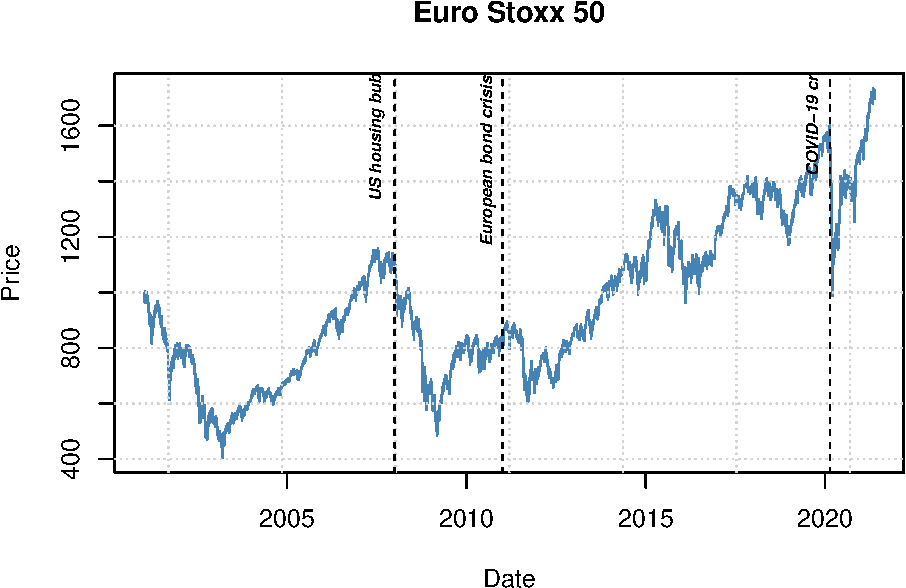
\includegraphics[width=1\linewidth]{_main_files/figure-latex/plot1-1} 

}

\caption{Eurostoxx 50 Price Index prices}\label{fig:plot1}
\end{figure}

\newpage

In figure \ref{fig:plot2} the daily log-returns are visualized. A stylized fact that is observable is the volatility clustering. As can be seen: periods of large volatility are mostly followed by large volatility and small volatility by small volatility.

\begin{figure}[h]

{\centering 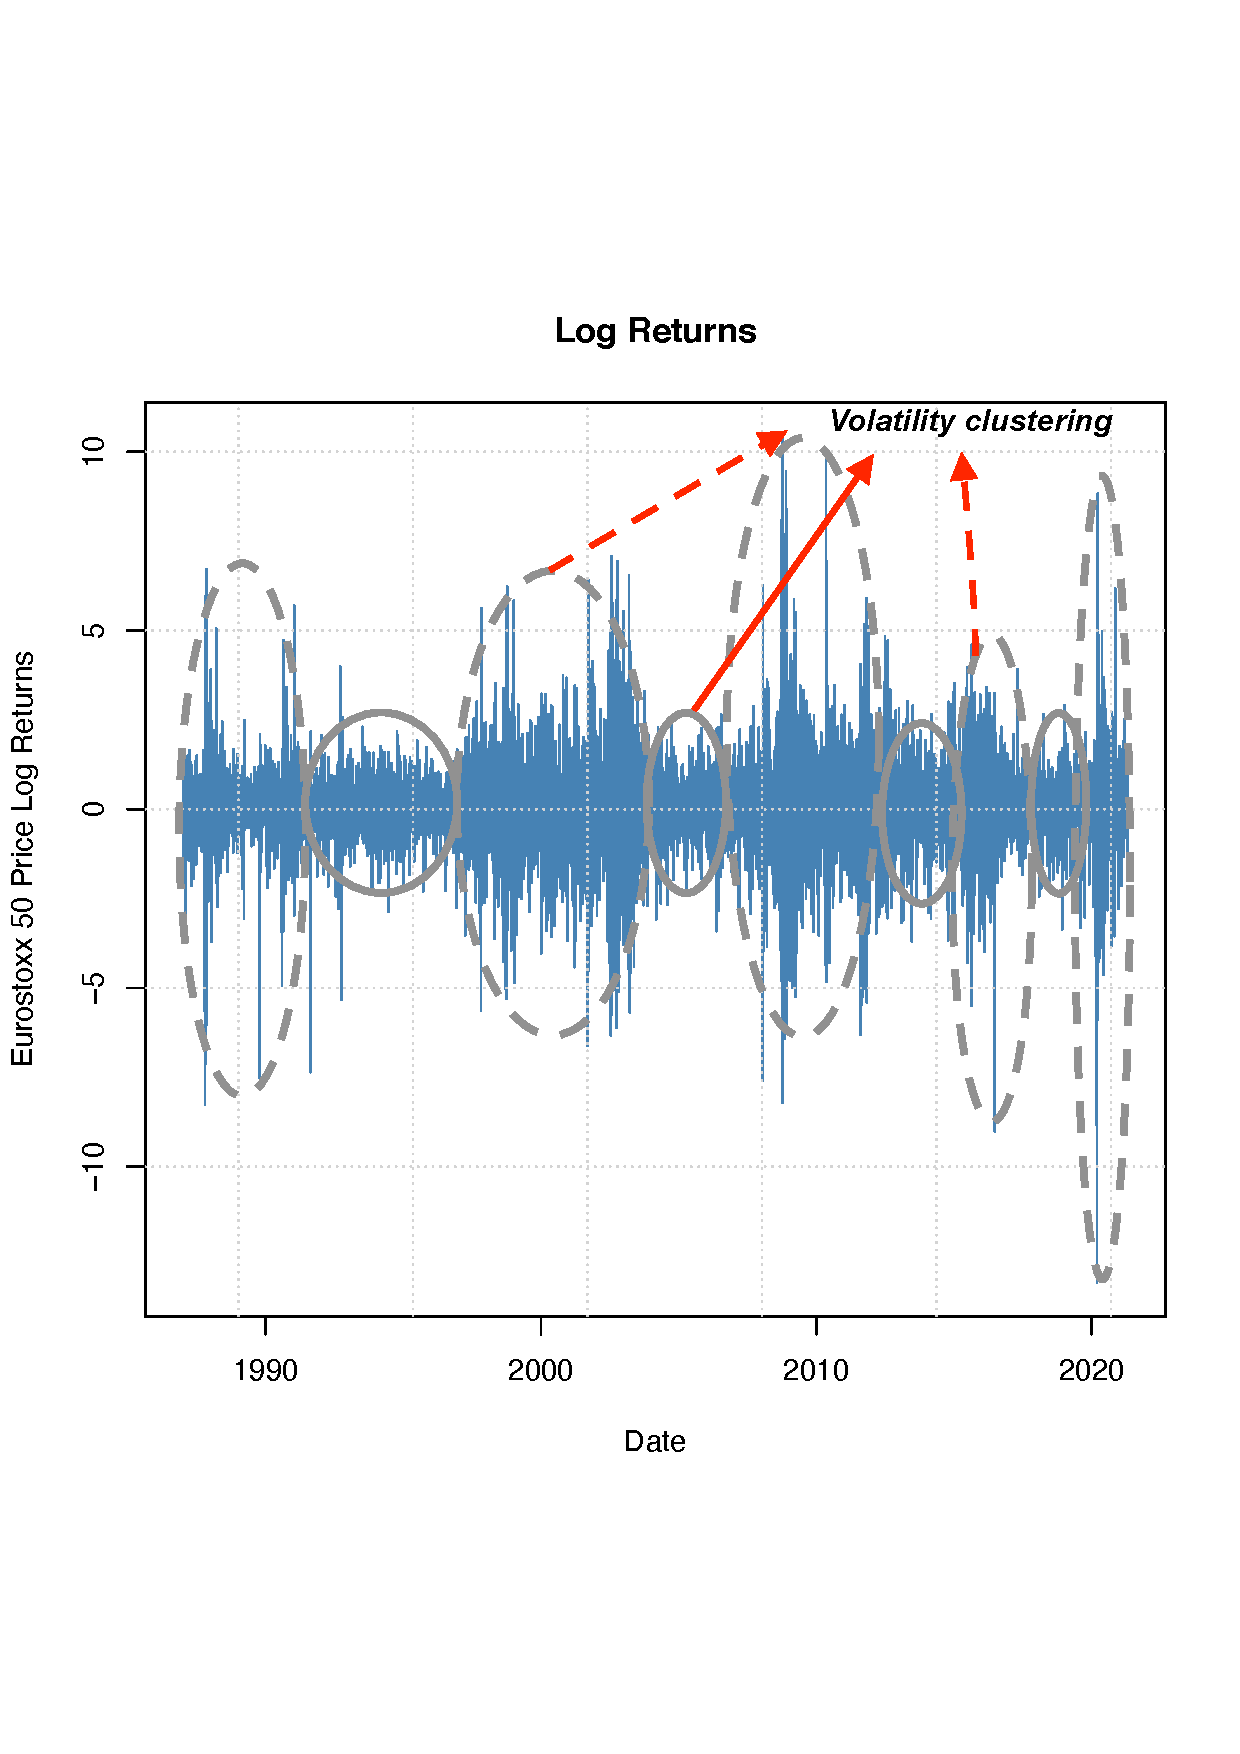
\includegraphics[width=0.75\linewidth]{figures/vol-clustering-final-withcircles} 

}

\caption{Eurostoxx 50 Price Index log returns}\label{fig:plot2}
\end{figure}

\begin{figure}[h]

{\centering 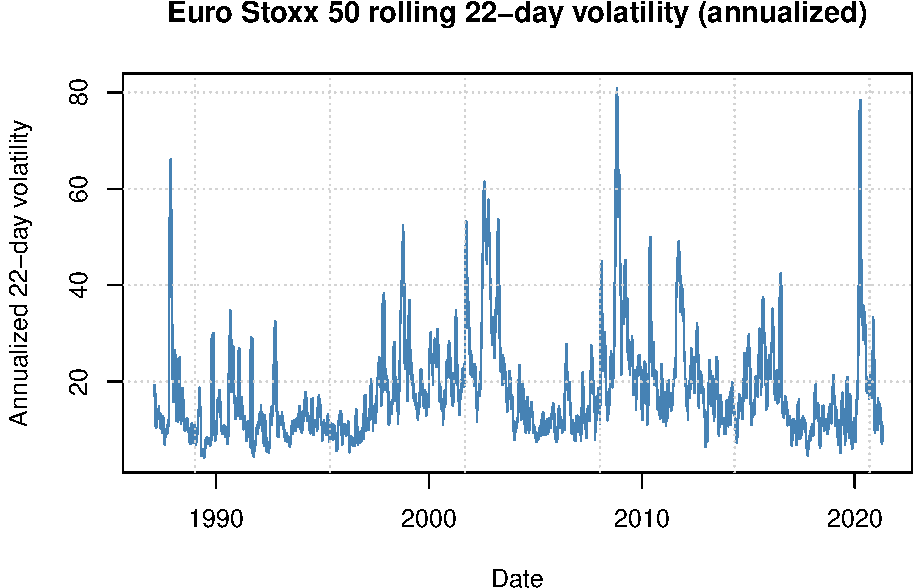
\includegraphics[width=0.75\linewidth]{_main_files/figure-latex/plot3-1} 

}

\caption{Eurostoxx 50 rolling volatility (22 days, calculated over 252 days)}\label{fig:plot3}
\end{figure}

\newpage

In figure \ref{fig:plot4} the density distribution of the log returns are examined. As can be seen, as already mentioned in part \ref{styl-facts}, log returns are not really normally distributed. So

\begin{figure}

{\centering 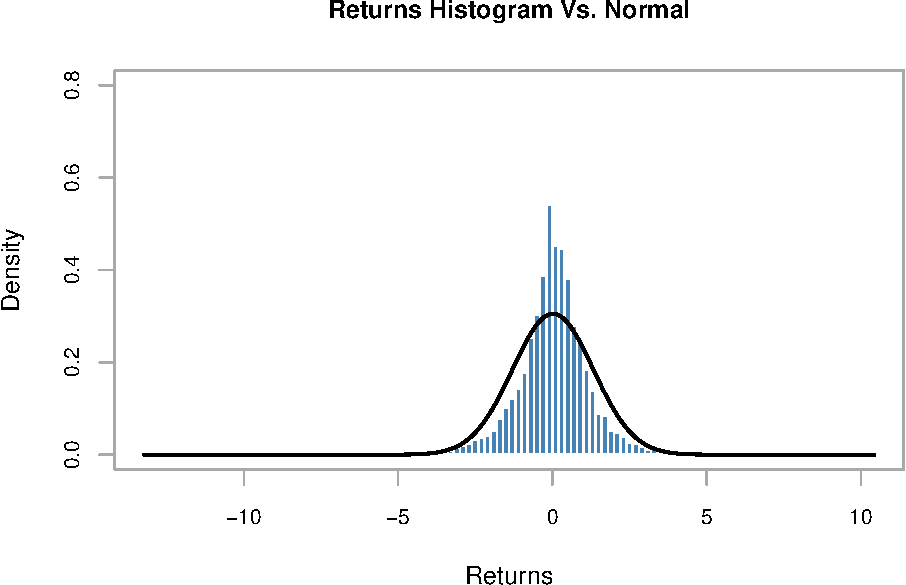
\includegraphics[width=0.75\linewidth]{_main_files/figure-latex/plot4-1} 

}

\caption{Density vs. Normal Eurostoxx 50 log returns)}\label{fig:plot4}
\end{figure}

\newpage

ACF plots: to do\ldots{}

\begin{figure}[h]

{\centering 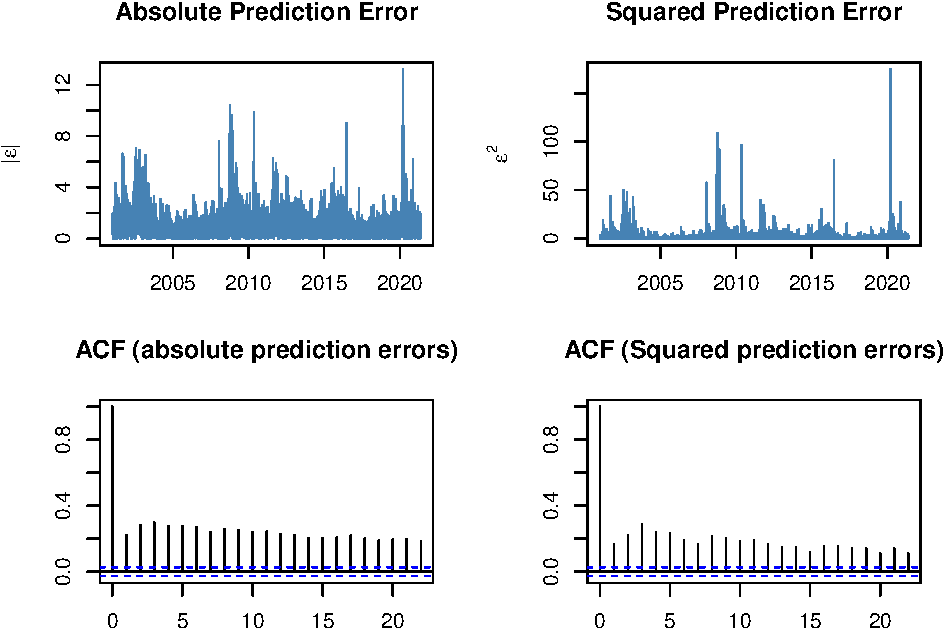
\includegraphics[width=0.75\linewidth]{_main_files/figure-latex/acfplots-1} 

}

\caption{Absolute prediction errors}\label{fig:acfplots}
\end{figure}

\clearpage

\hypertarget{methodology}{%
\section{Methodology}\label{methodology}}

\hypertarget{garch-models}{%
\subsection{Garch models}\label{garch-models}}

As already mentioned in \ldots, GARCH models GARCH, EGARCH, IGARCH, GJRGARCH, NGARCH, TGARCH and NAGARCH (or TSGARCH) will be estimated. Additionally the distributions will be examined as well, including the normal, student-t distribution, skewed student-t distribution, generalized error distribution, skewed generalized error distribution and the skewed generalized t distribution. ~\\

They will be estimated using maximum likelihood. As already mentioned, fortunately, Alexios \textcite{alexios2020} has made it easy for us to implement this methodology in the R language (v.3.6.1) with the package ``rugarch'' v.1.4-4 (\emph{R univariate garch}), which gives us a bit more time to focus on the results and the interpretation.~\\

Maximum likelihood estimation is a method to find the distribution parameters that best fit the observed data, through maximization of the likelihood function, or the computationally more efficient log-likelihood function (by taking the natural logarithm). It is assumed that the return data is i.i.d. and that there is some underlying parametrized density function \(f\) with one or more parameters that generate the data, defined as a vector \(\theta\) (\eqref{eq:pdf}). These functions are based on the joint probability distribution of the observed data (equation \eqref{eq:logl}). Subsequently, the (log)likelihood function is maximized using an optimization algorithm (equation \eqref{eq:optim}).~\\

\begin{align} 
  y_1,y_2,...,y_N \sim i.i.d
    \\
  y_i \sim f(y|\theta)
 \label{eq:pdf}
\end{align}

\begin{align} 
 L(\theta) = \prod^N_{i=1}f(y_i|\theta)
  \\
 \log(L(\theta)) = \sum^N_{i=1} \log f(y_i |\theta)
 \label{eq:logl}
\end{align}

\begin{align} 
\theta^{*} = arg \max_{\theta} [ L] \\
\theta^{*} = arg \max_{\theta} [\log(L)]
 \label{eq:optim}
\end{align}

\hypertarget{acd-models-meth}{%
\subsection{ACD models}\label{acd-models-meth}}

Following \textcite{ghalanos2016}, arguments of ACD models are specified as in \textcite{hansen1994}. The density function \(f(y|\alpha)\) has parameters \(\alpha_t = (\mu_t, \sigma_t, \nu_t)\), with equation \eqref{eq:cmean}, the conditional mean equation. Equation \eqref{eq:cvariance} as the conditional variance. And \(\nu_t=\nu(\theta,x_t)\) the remaining parameters of the distribution like the skewness and kurtosis (shape) parameters.

\begin{align} 
\mu_{t}=\mu\left(\theta, x_{t}\right)=E\left(y_{t} \mid x_{t}\right)
 \label{eq:cmean}
\end{align}

\begin{align}
\sigma_{t}^{2}=\sigma^{2}\left(\theta, x_{t}\right)=E\left(\left(y_{t}-\mu_{t}^{2}\right) \mid x_{t}\right)
 \label{eq:cvariance}
\end{align}

To further explain the difference between GARCH and ACD. The scaled innovations are given by equation \eqref{eq:scaledinn}. The conditional density is given by equation \eqref{eq:conddens} and related to the density function \(f(y|\alpha)\) as in equation \eqref{eq:densityconddens}.

\begin{align}
z_{t}(\theta)=\frac{y_{t}-\mu\left(\theta, x_{t}\right)}{\sigma\left(\theta, x_{t}\right)}
\label{eq:scaledinn}
\end{align}

\begin{align}
g\left(z \mid \eta_{t}\right)=\frac{d}{d z} P\left(z_{t}<z \mid \eta_{t}\right)
\label{eq:conddens}
\end{align}

\begin{align}
f\left(y_{t} \mid \mu_{t}, \sigma_{t}^{2}, \eta_{t}\right)=\frac{1}{\sigma_{t}} g\left(z_{t} \mid \eta_{t}\right)
\end{align}
\label{eq:densityconddens}

Again \textcite{ghalanos2016} makes it easier to implement the somewhat complex ACD models using the R language with package ``racd''.

\hypertarget{control-tests}{%
\subsection{Control Tests}\label{control-tests}}

\hypertarget{unconditional-coverage-test-of-kupiec1995}{%
\subsubsection{\texorpdfstring{Unconditional coverage test of \textcite{kupiec1995}}{Unconditional coverage test of @kupiec1995}}\label{unconditional-coverage-test-of-kupiec1995}}

A number of tests are computed to see if the value-at-risk estimations capture the actual losses well. A first one is the unconditional coverage test by \textcite{kupiec1995}. The unconditional coverage or proportion of failures method tests if the actual value-at-risk exceedances are consistent with the expected exceedances (a chosen percentile, e.g.~1\% percentile) of the VaR model. Following \textcite{kupiec1995} and \textcite{ghalanos2020}, the number of exceedence follow a binomial distribution (with thus probability equal to the significance level or expected proportion) under the null hypothesis of a correct VaR model. The test is conducted as a likelihood ratio test with statistic like in equation \eqref{eq:uccov}, with \(p\) the probability of an exceedence for a confidence level, \(N\) the sample size and \(X\) the number of exceedence. The null hypothesis states that the test statistic \(L R^{u c}\) is \(\chi^2\)-distributed with one degree of freedom or that the probability of failure \(\hat p\) is equal to the chosen percentile \(\alpha\).

\begin{align}
L R^{u c}=-2 \ln \left(\frac{(1-p)^{N-X} p^{X}}{\left(1-\frac{X}{N}\right)^{N-X}\left(\frac{X}{N}\right)^{X}}\right)
\label{eq:uccov}
\end{align}

\hypertarget{conditional-coverage-test-of-christoffersen2001}{%
\subsubsection{\texorpdfstring{Conditional coverage test of \textcite{christoffersen2001}}{Conditional coverage test of @christoffersen2001}}\label{conditional-coverage-test-of-christoffersen2001}}

\textcite{christoffersen2001} proposed the conditional coverage test. It is tests for unconditional covrage and serial independence. The serial independence is important while the \(L R^{u c}\) can give a false picture while at any point in time it classifies inaccurate VaR estimates as ``acceptably accurate'' \autocite{bali2007}. For a certain VaR estimate an indicator variable, \(I_t(\alpha)\), is computed as equation \eqref{eq:ccov}.

\begin{align}
I_{t}(\alpha)=\left\{\begin{array}{ll}
1 & \text { if exceedence occurs } \\
0 & \text { if no exceedence occurs }
\end{array} .\right.
\label{eq:ccov}
\end{align}

It involves a likelihood ratio test's null hypothesis is that the statistic is \(\chi^2\)-distributed with two degrees of freedom or that the probability of violation \(\hat p\) (unconditional coverage) as well as the conditional coverage (independence) is equal to the chosen percentile \(\alpha\).

\hypertarget{dynamic-quantile-test}{%
\subsubsection{Dynamic quantile test}\label{dynamic-quantile-test}}

\textcite{engle1999} with the aim to provide completeness to the conditional coverage test of \textcite{christoffersen2001} developed the Dynamic quantile test. It consists in testing some restriction in a \ldots(work-in-progress).

\clearpage

\hypertarget{analysis}{%
\chapter{Empirical Findings}\label{analysis}}

\minitoc 

\hypertarget{density-of-the-returns}{%
\section{Density of the returns}\label{density-of-the-returns}}

\#\#MLE distribution parameters

\begin{Shaded}
\begin{Highlighting}[]
\NormalTok{sgt.mle2 }\OtherTok{\textless{}{-}} \ControlFlowTok{function}\NormalTok{ (X.f, }\AttributeTok{mu.f =}\NormalTok{ mu }\SpecialCharTok{\textasciitilde{}}\NormalTok{ mu, }\AttributeTok{sigma.f =}\NormalTok{ sigma }\SpecialCharTok{\textasciitilde{}}\NormalTok{ sigma, }\AttributeTok{lambda.f =}\NormalTok{ lambda }\SpecialCharTok{\textasciitilde{}} 
\NormalTok{            lambda, }\AttributeTok{p.f =}\NormalTok{ p }\SpecialCharTok{\textasciitilde{}}\NormalTok{ p, }\AttributeTok{q.f =}\NormalTok{ q }\SpecialCharTok{\textasciitilde{}}\NormalTok{ q, }\AttributeTok{data =} \FunctionTok{parent.frame}\NormalTok{(), }
\NormalTok{          start, subset, }\AttributeTok{method =} \StringTok{"BFGS"}\NormalTok{, }\AttributeTok{itnmax =} \ConstantTok{NULL}\NormalTok{, }
          \AttributeTok{hessian.method =} \StringTok{"Richardson"}\NormalTok{, }\AttributeTok{gradient.method =} \StringTok{"Richardson"}\NormalTok{, }
          \AttributeTok{mean.cent =} \ConstantTok{TRUE}\NormalTok{, }\AttributeTok{var.adj =} \ConstantTok{TRUE}\NormalTok{, ..., }\AttributeTok{lower =}\SpecialCharTok{{-}}\ConstantTok{Inf}\NormalTok{, }\AttributeTok{upper=}\ConstantTok{Inf}\NormalTok{) \{}
\NormalTok{  formList }\OtherTok{=} \FunctionTok{list}\NormalTok{(}\AttributeTok{X =}\NormalTok{ X.f, }\AttributeTok{mu =}\NormalTok{ mu.f, }\AttributeTok{sigma =}\NormalTok{ sigma.f, }\AttributeTok{lambda =}\NormalTok{ lambda.f, }
                  \AttributeTok{p =}\NormalTok{ p.f, }\AttributeTok{q =}\NormalTok{ q.f)}
\NormalTok{  varNames }\OtherTok{=} \ConstantTok{NULL}
\NormalTok{  envir }\OtherTok{=} \FunctionTok{new.env}\NormalTok{()}
  \ControlFlowTok{for}\NormalTok{ (i }\ControlFlowTok{in} \DecValTok{1}\SpecialCharTok{:}\DecValTok{6}\NormalTok{) \{}
\NormalTok{    formList[[i]] }\OtherTok{=}\NormalTok{ stats}\SpecialCharTok{::}\FunctionTok{as.formula}\NormalTok{(formList[[i]])}
    \ControlFlowTok{if}\NormalTok{ (}\FunctionTok{length}\NormalTok{(formList[[i]]) }\SpecialCharTok{==}\NormalTok{ 2L) \{}
\NormalTok{      formList[[i]][[3L]] }\OtherTok{=}\NormalTok{ formList[[i]][[2L]]}
\NormalTok{      formList[[i]][[2L]] }\OtherTok{=} \FunctionTok{as.name}\NormalTok{(}\FunctionTok{names}\NormalTok{(formList)[i])}
\NormalTok{    \}}
    \ControlFlowTok{else} \ControlFlowTok{if}\NormalTok{ (}\FunctionTok{as.character}\NormalTok{(formList[[i]][[2L]]) }\SpecialCharTok{!=} \FunctionTok{names}\NormalTok{(formList)[i]) \{}
      \FunctionTok{warning}\NormalTok{(}\FunctionTok{paste}\NormalTok{(}\StringTok{"The left hand side of "}\NormalTok{, }\FunctionTok{names}\NormalTok{(formList)[i], }
                    \StringTok{".f was changed from "}\NormalTok{, }\FunctionTok{as.character}\NormalTok{(formList[[i]][[2L]]), }
                    \StringTok{" to "}\NormalTok{, }\FunctionTok{names}\NormalTok{(formList)[i], }\AttributeTok{sep =} \StringTok{""}\NormalTok{))}
\NormalTok{    \}}
\NormalTok{    varNames }\OtherTok{=} \FunctionTok{c}\NormalTok{(varNames, }\FunctionTok{all.vars}\NormalTok{(formList[[i]][[3L]]))}
\NormalTok{  \}}
  \ControlFlowTok{if}\NormalTok{ (}\FunctionTok{class}\NormalTok{(data)[1L] }\SpecialCharTok{==} \StringTok{"matrix"}\NormalTok{) }
\NormalTok{    data }\OtherTok{=} \FunctionTok{as.data.frame}\NormalTok{(data)}
  \ControlFlowTok{if}\NormalTok{ (}\SpecialCharTok{!}\FunctionTok{is.list}\NormalTok{(data) }\SpecialCharTok{\&\&} \SpecialCharTok{!}\FunctionTok{is.environment}\NormalTok{(data)) }
    \FunctionTok{stop}\NormalTok{(}\StringTok{"\textquotesingle{}data\textquotesingle{} must be a list or an environment"}\NormalTok{)}
\NormalTok{  start }\OtherTok{=} \FunctionTok{as.list}\NormalTok{(start)}
  \ControlFlowTok{if}\NormalTok{ (}\FunctionTok{is.null}\NormalTok{(}\FunctionTok{names}\NormalTok{(start))) }
    \FunctionTok{stop}\NormalTok{(}\StringTok{"\textquotesingle{}start\textquotesingle{} must be a named list or named numeric vector"}\NormalTok{)}
  \ControlFlowTok{if}\NormalTok{ (}\StringTok{""} \SpecialCharTok{\%in\%} \FunctionTok{names}\NormalTok{(start)) }
    \FunctionTok{stop}\NormalTok{(}\StringTok{"at least one of the elements in \textquotesingle{}start\textquotesingle{} is missing a name"}\NormalTok{)}
\NormalTok{  parNames }\OtherTok{=} \FunctionTok{names}\NormalTok{(start)}
\NormalTok{  varNames }\OtherTok{=}\NormalTok{ varNames[}\FunctionTok{is.na}\NormalTok{(}\FunctionTok{match}\NormalTok{(varNames, parNames))]}
  \ControlFlowTok{if}\NormalTok{ (}\FunctionTok{length}\NormalTok{(varNames) }\SpecialCharTok{==}\NormalTok{ 0L) }
    \FunctionTok{stop}\NormalTok{(}\StringTok{"there is no reference to data in the given formulas"}\NormalTok{)}
  \ControlFlowTok{for}\NormalTok{ (i }\ControlFlowTok{in}\NormalTok{ varNames) \{}
    \ControlFlowTok{if}\NormalTok{ (}\SpecialCharTok{!}\FunctionTok{exists}\NormalTok{(i, data)) }
      \FunctionTok{stop}\NormalTok{(}\FunctionTok{paste}\NormalTok{(i, }\StringTok{"is not contained in \textquotesingle{}start\textquotesingle{} and it is not found in \textquotesingle{}data\textquotesingle{}"}\NormalTok{))}
    \FunctionTok{assign}\NormalTok{(i, }\FunctionTok{eval}\NormalTok{(}\FunctionTok{parse}\NormalTok{(}\AttributeTok{text =} \FunctionTok{paste}\NormalTok{(}\StringTok{"as.numeric(data$"}\NormalTok{, }
\NormalTok{                                      i, }\StringTok{")"}\NormalTok{, }\AttributeTok{sep =} \StringTok{""}\NormalTok{))), envir)}
\NormalTok{  \}}
  \ControlFlowTok{if}\NormalTok{ (}\FunctionTok{length}\NormalTok{(varNames) }\SpecialCharTok{\textgreater{}} \DecValTok{1}\NormalTok{) \{}
    \ControlFlowTok{for}\NormalTok{ (i }\ControlFlowTok{in} \DecValTok{2}\SpecialCharTok{:}\FunctionTok{length}\NormalTok{(varNames)) \{}
      \ControlFlowTok{if}\NormalTok{ (}\FunctionTok{length}\NormalTok{(}\FunctionTok{eval}\NormalTok{(}\FunctionTok{parse}\NormalTok{(}\AttributeTok{text =} \FunctionTok{paste}\NormalTok{(}\StringTok{"envir$"}\NormalTok{, varNames[1L], }
                                         \AttributeTok{sep =} \StringTok{""}\NormalTok{)))) }\SpecialCharTok{!=} \FunctionTok{length}\NormalTok{(}\FunctionTok{eval}\NormalTok{(}\FunctionTok{parse}\NormalTok{(}\AttributeTok{text =} \FunctionTok{paste}\NormalTok{(}\StringTok{"envir$"}\NormalTok{, }
\NormalTok{                                                                                        varNames[i], }\AttributeTok{sep =} \StringTok{""}\NormalTok{))))) }
        \FunctionTok{stop}\NormalTok{(}\FunctionTok{paste}\NormalTok{(}\StringTok{"the length of the variable"}\NormalTok{, varNames[i], }
                   \StringTok{"does not match the length of the variable"}\NormalTok{, }
\NormalTok{                   varNames[1L]))}
\NormalTok{    \}}
\NormalTok{  \}}
\NormalTok{  control }\OtherTok{=} \FunctionTok{list}\NormalTok{(...)}
  \ControlFlowTok{if}\NormalTok{ (}\SpecialCharTok{!}\FunctionTok{is.null}\NormalTok{(control}\SpecialCharTok{$}\NormalTok{maximize)) }
    \FunctionTok{stop}\NormalTok{(}\StringTok{"\textquotesingle{}maximize\textquotesingle{} option not allowed"}\NormalTok{)}
  \ControlFlowTok{if}\NormalTok{ (}\SpecialCharTok{!}\FunctionTok{missing}\NormalTok{(subset)) }
    \ControlFlowTok{for}\NormalTok{ (i }\ControlFlowTok{in}\NormalTok{ varNames) }\FunctionTok{assign}\NormalTok{(i, }\FunctionTok{eval}\NormalTok{(}\FunctionTok{parse}\NormalTok{(}\AttributeTok{text =} \FunctionTok{paste}\NormalTok{(}\StringTok{"envir$"}\NormalTok{, }
\NormalTok{                                                          i, }\StringTok{"[subset]"}\NormalTok{, }\AttributeTok{sep =} \StringTok{""}\NormalTok{))), envir)}
\NormalTok{  keep }\OtherTok{=} \FunctionTok{rep}\NormalTok{(}\ConstantTok{TRUE}\NormalTok{, }\FunctionTok{length}\NormalTok{(}\FunctionTok{eval}\NormalTok{(}\FunctionTok{parse}\NormalTok{(}\AttributeTok{text =} \FunctionTok{paste}\NormalTok{(}\StringTok{"envir$"}\NormalTok{, }
\NormalTok{                                                  varNames[1L], }\AttributeTok{sep =} \StringTok{""}\NormalTok{)))))}
  \ControlFlowTok{for}\NormalTok{ (i }\ControlFlowTok{in}\NormalTok{ varNames) keep }\OtherTok{=}\NormalTok{ keep }\SpecialCharTok{\&} \FunctionTok{is.finite}\NormalTok{(}\FunctionTok{eval}\NormalTok{(}\FunctionTok{parse}\NormalTok{(}\AttributeTok{text =} \FunctionTok{paste}\NormalTok{(}\StringTok{"envir$"}\NormalTok{, }
\NormalTok{                                                                      i, }\AttributeTok{sep =} \StringTok{""}\NormalTok{))))}
  \ControlFlowTok{for}\NormalTok{ (i }\ControlFlowTok{in}\NormalTok{ varNames) }\FunctionTok{assign}\NormalTok{(i, }\FunctionTok{eval}\NormalTok{(}\FunctionTok{parse}\NormalTok{(}\AttributeTok{text =} \FunctionTok{paste}\NormalTok{(}\StringTok{"envir$"}\NormalTok{, }
\NormalTok{                                                        i, }\StringTok{"[keep]"}\NormalTok{, }\AttributeTok{sep =} \StringTok{""}\NormalTok{))), envir)}
\NormalTok{  loglik }\OtherTok{=} \ControlFlowTok{function}\NormalTok{(params) \{}
    \ControlFlowTok{for}\NormalTok{ (i }\ControlFlowTok{in} \DecValTok{1}\SpecialCharTok{:}\FunctionTok{length}\NormalTok{(parNames)) }\FunctionTok{assign}\NormalTok{(parNames[i], }\FunctionTok{unlist}\NormalTok{(params[i]))}
\NormalTok{    X }\OtherTok{=} \FunctionTok{eval}\NormalTok{(formList[[1L]][[3L]])}
\NormalTok{    mu }\OtherTok{=} \FunctionTok{eval}\NormalTok{(formList[[2L]][[3L]])}
\NormalTok{    sigma }\OtherTok{=} \FunctionTok{eval}\NormalTok{(formList[[3L]][[3L]])}
\NormalTok{    lambda }\OtherTok{=} \FunctionTok{eval}\NormalTok{(formList[[4L]][[3L]])}
\NormalTok{    p }\OtherTok{=} \FunctionTok{eval}\NormalTok{(formList[[5L]][[3L]])}
\NormalTok{    q }\OtherTok{=} \FunctionTok{eval}\NormalTok{(formList[[6L]][[3L]])}
    \FunctionTok{sum}\NormalTok{(}\FunctionTok{dsgt}\NormalTok{(X, mu, sigma, lambda, p, q, mean.cent, var.adj, }
             \AttributeTok{log =} \ConstantTok{TRUE}\NormalTok{))}
\NormalTok{  \}}
  \FunctionTok{environment}\NormalTok{(loglik) }\OtherTok{=}\NormalTok{ envir}
\NormalTok{  negloglik }\OtherTok{=} \ControlFlowTok{function}\NormalTok{(params) \{}
    \SpecialCharTok{{-}}\FunctionTok{loglik}\NormalTok{(params)}
\NormalTok{  \}}
  \ControlFlowTok{if}\NormalTok{ (}\SpecialCharTok{!}\FunctionTok{is.finite}\NormalTok{(}\FunctionTok{loglik}\NormalTok{(start))) }
    \FunctionTok{stop}\NormalTok{(}\StringTok{"\textquotesingle{}start\textquotesingle{} yields infinite or non{-}computable SGT function values"}\NormalTok{)}
\NormalTok{  optimum }\OtherTok{=} \FunctionTok{suppressWarnings}\NormalTok{(optimx}\SpecialCharTok{::}\FunctionTok{optimx}\NormalTok{(}\AttributeTok{par =} \FunctionTok{unlist}\NormalTok{(start), }
                                            \AttributeTok{fn =}\NormalTok{ negloglik, }\AttributeTok{method =}\NormalTok{ method, }\AttributeTok{itnmax =}\NormalTok{ itnmax, }\AttributeTok{control =}\NormalTok{ control, }\AttributeTok{lower=}\NormalTok{lower, }\AttributeTok{upper=}\NormalTok{upper))}
\NormalTok{  minimum }\OtherTok{=} \FunctionTok{min}\NormalTok{(optimum}\SpecialCharTok{$}\NormalTok{value, }\AttributeTok{na.rm =} \ConstantTok{TRUE}\NormalTok{)}
  \ControlFlowTok{if}\NormalTok{ (}\SpecialCharTok{!}\FunctionTok{is.finite}\NormalTok{(minimum)) }
    \FunctionTok{stop}\NormalTok{(}\StringTok{"All Maximization Methods Failed"}\NormalTok{)}
\NormalTok{  whichbest }\OtherTok{=} \FunctionTok{max}\NormalTok{(}\FunctionTok{which}\NormalTok{(minimum }\SpecialCharTok{==}\NormalTok{ optimum}\SpecialCharTok{$}\NormalTok{value))}
\NormalTok{  optimal }\OtherTok{=}\NormalTok{ optimum[whichbest, ]}
\NormalTok{  estimate }\OtherTok{=} \FunctionTok{as.numeric}\NormalTok{(optimum[whichbest, }\DecValTok{1}\SpecialCharTok{:}\FunctionTok{length}\NormalTok{(parNames)])}
  \FunctionTok{names}\NormalTok{(estimate) }\OtherTok{=}\NormalTok{ parNames}
\NormalTok{  H }\OtherTok{=} \FunctionTok{tryCatch}\NormalTok{(numDeriv}\SpecialCharTok{::}\FunctionTok{hessian}\NormalTok{(loglik, estimate, }\AttributeTok{method =}\NormalTok{ hessian.method), }
               \AttributeTok{error =} \ControlFlowTok{function}\NormalTok{(e) \{}
                 \FunctionTok{warning}\NormalTok{(}\StringTok{"hessian matrix calculation failed"}\NormalTok{)}
                 \FunctionTok{return}\NormalTok{(}\FunctionTok{as.matrix}\NormalTok{(}\ConstantTok{NaN}\NormalTok{))}
\NormalTok{               \})}
\NormalTok{  varcov }\OtherTok{=} \FunctionTok{tryCatch}\NormalTok{(}\SpecialCharTok{{-}}\FunctionTok{qr.solve}\NormalTok{(H), }\AttributeTok{error =} \ControlFlowTok{function}\NormalTok{(e) \{}
    \FunctionTok{warning}\NormalTok{(}\StringTok{"covariance matrix calculation failed due to a problem with the hessian"}\NormalTok{)}
    \FunctionTok{return}\NormalTok{(}\FunctionTok{as.matrix}\NormalTok{(}\ConstantTok{NaN}\NormalTok{))}
\NormalTok{  \})}
\NormalTok{  std.error }\OtherTok{=} \FunctionTok{sqrt}\NormalTok{(}\FunctionTok{diag}\NormalTok{(varcov))}
  \ControlFlowTok{if}\NormalTok{ (}\FunctionTok{is.finite}\NormalTok{(varcov[}\DecValTok{1}\NormalTok{, }\DecValTok{1}\NormalTok{])) }
    \FunctionTok{names}\NormalTok{(std.error) }\OtherTok{=}\NormalTok{ parNames}
\NormalTok{  gradient }\OtherTok{=} \FunctionTok{tryCatch}\NormalTok{(numDeriv}\SpecialCharTok{::}\FunctionTok{grad}\NormalTok{(loglik, estimate, }\AttributeTok{method =}\NormalTok{ gradient.method), }
                      \AttributeTok{error =} \ControlFlowTok{function}\NormalTok{(e) \{}
                        \FunctionTok{warning}\NormalTok{(}\StringTok{"gradient calculation failed"}\NormalTok{)}
                        \FunctionTok{return}\NormalTok{(}\ConstantTok{NaN}\NormalTok{)}
\NormalTok{                      \})}
\NormalTok{  result }\OtherTok{=} \FunctionTok{list}\NormalTok{(}\AttributeTok{maximum =} \SpecialCharTok{{-}}\NormalTok{minimum, }\AttributeTok{estimate =}\NormalTok{ estimate, }\AttributeTok{convcode =} \FunctionTok{as.numeric}\NormalTok{(optimal}\SpecialCharTok{$}\NormalTok{convcode), }
                \AttributeTok{niter =} \FunctionTok{as.numeric}\NormalTok{(optimal}\SpecialCharTok{$}\NormalTok{niter), }\AttributeTok{best.method.used =} \FunctionTok{row.names}\NormalTok{(optimal), }
                \AttributeTok{optimx =}\NormalTok{ optimum, }\AttributeTok{hessian =}\NormalTok{ H, }\AttributeTok{gradient =}\NormalTok{ gradient, }
                \AttributeTok{varcov =}\NormalTok{ varcov, }\AttributeTok{std.error =}\NormalTok{ std.error)}
  \FunctionTok{class}\NormalTok{(result) }\OtherTok{=} \FunctionTok{c}\NormalTok{(}\StringTok{"sgtest"}\NormalTok{, }\FunctionTok{class}\NormalTok{(result))}
  \FunctionTok{return}\NormalTok{(result)}
\NormalTok{\}}
\end{Highlighting}
\end{Shaded}

\begin{Shaded}
\begin{Highlighting}[]
\FunctionTok{library}\NormalTok{(sgt)}
\FunctionTok{require}\NormalTok{(graphics)}
\FunctionTok{require}\NormalTok{(stats)}


\NormalTok{DistMLE }\OtherTok{\textless{}{-}} \ControlFlowTok{function}\NormalTok{(series) \{}
  
  \DocumentationTok{\#\#\# SGT}
\NormalTok{  X.data }\OtherTok{\textless{}{-}}\NormalTok{ X }\SpecialCharTok{\textasciitilde{}} \FunctionTok{coredata}\NormalTok{(series)}
  
\NormalTok{  SGT\_start }\OtherTok{\textless{}{-}} \FunctionTok{list}\NormalTok{(}\AttributeTok{mu =} \DecValTok{0}\NormalTok{, }\AttributeTok{sigma =} \DecValTok{2}\NormalTok{, }\AttributeTok{lambda =} \DecValTok{0}\NormalTok{, }\AttributeTok{p =} \DecValTok{2}\NormalTok{, }\AttributeTok{q =} \DecValTok{12}\NormalTok{)}
\NormalTok{  SGT\_result }\OtherTok{\textless{}{-}} \FunctionTok{sgt.mle2}\NormalTok{(}\AttributeTok{X.f =}\NormalTok{ X.data, }\AttributeTok{start =}\NormalTok{ SGT\_start)}
\NormalTok{  SGT\_sumResult }\OtherTok{\textless{}{-}} \FunctionTok{summary}\NormalTok{(SGT\_result)}
\NormalTok{  SGT\_AIC }\OtherTok{\textless{}{-}} \DecValTok{2}\SpecialCharTok{*}\FunctionTok{length}\NormalTok{(SGT\_result}\SpecialCharTok{$}\NormalTok{estimate) }\SpecialCharTok{{-}} \DecValTok{2}\SpecialCharTok{*}\NormalTok{SGT\_sumResult}\SpecialCharTok{$}\NormalTok{maximum}
  
  \DocumentationTok{\#\#\# SGT plot fit}
\NormalTok{  xvals }\OtherTok{=} \FunctionTok{seq}\NormalTok{(}\SpecialCharTok{{-}}\DecValTok{3}\NormalTok{,}\DecValTok{3}\NormalTok{,}\AttributeTok{by=}\FloatTok{0.01}\NormalTok{)}
\NormalTok{  SGT\_mu }\OtherTok{\textless{}{-}}\NormalTok{ SGT\_result}\SpecialCharTok{$}\NormalTok{estimate[}\DecValTok{1}\NormalTok{]}
\NormalTok{  SGT\_sigma }\OtherTok{\textless{}{-}}\NormalTok{ SGT\_result}\SpecialCharTok{$}\NormalTok{estimate[}\DecValTok{2}\NormalTok{]}
\NormalTok{  SGT\_lambda }\OtherTok{\textless{}{-}}\NormalTok{ SGT\_result}\SpecialCharTok{$}\NormalTok{estimate[}\DecValTok{3}\NormalTok{]}
\NormalTok{  SGT\_p }\OtherTok{\textless{}{-}}\NormalTok{ SGT\_result}\SpecialCharTok{$}\NormalTok{estimate[}\DecValTok{4}\NormalTok{]}
\NormalTok{  SGT\_q }\OtherTok{\textless{}{-}}\NormalTok{ SGT\_result}\SpecialCharTok{$}\NormalTok{estimate[}\DecValTok{5}\NormalTok{]}
  \FunctionTok{plot}\NormalTok{(xvals, }\FunctionTok{dsgt}\NormalTok{(xvals, }\AttributeTok{mu =}\NormalTok{ SGT\_mu, }\AttributeTok{sigma =}\NormalTok{ SGT\_sigma, }\AttributeTok{lambda =}\NormalTok{ SGT\_lambda, }\AttributeTok{p =}\NormalTok{ SGT\_p, }\AttributeTok{q =}\NormalTok{ SGT\_q), }\AttributeTok{col=}\StringTok{"red"}\NormalTok{, }\AttributeTok{type =}\StringTok{"l"}\NormalTok{,}\AttributeTok{main =} \StringTok{"SGT (sgt.mle2)"}\NormalTok{)}
  \FunctionTok{lines}\NormalTok{(}\FunctionTok{density}\NormalTok{(}\FunctionTok{coredata}\NormalTok{(series)))}
  
  
  
  \DocumentationTok{\#\#\# SGED (sgt.mle2)}
  
\NormalTok{  SGED\_start }\OtherTok{\textless{}{-}} \FunctionTok{list}\NormalTok{(}\AttributeTok{mu =} \DecValTok{0}\NormalTok{, }\AttributeTok{sigma =} \DecValTok{2}\NormalTok{, }\AttributeTok{lambda =} \DecValTok{0}\NormalTok{, }\AttributeTok{p =} \DecValTok{2}\NormalTok{, }\AttributeTok{q =} \DecValTok{750}\NormalTok{)}
\NormalTok{  SGED\_result }\OtherTok{\textless{}{-}} \FunctionTok{sgt.mle2}\NormalTok{(}\AttributeTok{X.f =}\NormalTok{ X.data, }\AttributeTok{start =}\NormalTok{ SGED\_start, }\AttributeTok{lower =} \FunctionTok{c}\NormalTok{(}\SpecialCharTok{{-}}\ConstantTok{Inf}\NormalTok{, }\SpecialCharTok{{-}}\ConstantTok{Inf}\NormalTok{, }\SpecialCharTok{{-}}\ConstantTok{Inf}\NormalTok{, }\SpecialCharTok{{-}}\ConstantTok{Inf}\NormalTok{,}\FloatTok{749.9}\NormalTok{), }\AttributeTok{upper =} \FunctionTok{c}\NormalTok{(}\ConstantTok{Inf}\NormalTok{,}\ConstantTok{Inf}\NormalTok{,}\ConstantTok{Inf}\NormalTok{,}\ConstantTok{Inf}\NormalTok{,}\FloatTok{750.1}\NormalTok{))}
\NormalTok{  SGED\_sumResult }\OtherTok{\textless{}{-}} \FunctionTok{summary}\NormalTok{(SGED\_result)}
\NormalTok{  SGED\_AIC }\OtherTok{\textless{}{-}} \DecValTok{2}\SpecialCharTok{*}\FunctionTok{length}\NormalTok{(SGED\_result}\SpecialCharTok{$}\NormalTok{estimate}\DecValTok{{-}1}\NormalTok{) }\SpecialCharTok{{-}} \DecValTok{2}\SpecialCharTok{*}\NormalTok{SGED\_sumResult}\SpecialCharTok{$}\NormalTok{maximum}
  
  \DocumentationTok{\#\#\# SGED Plot fit (sgt.mle2)}
\NormalTok{  SGED\_mu }\OtherTok{\textless{}{-}}\NormalTok{ SGED\_result}\SpecialCharTok{$}\NormalTok{estimate[}\DecValTok{1}\NormalTok{]}
\NormalTok{  SGED\_sigma }\OtherTok{\textless{}{-}}\NormalTok{ SGED\_result}\SpecialCharTok{$}\NormalTok{estimate[}\DecValTok{2}\NormalTok{]}
\NormalTok{  SGED\_lambda }\OtherTok{\textless{}{-}}\NormalTok{ SGED\_result}\SpecialCharTok{$}\NormalTok{estimate[}\DecValTok{3}\NormalTok{]}
\NormalTok{  SGED\_p }\OtherTok{\textless{}{-}}\NormalTok{ SGED\_result}\SpecialCharTok{$}\NormalTok{estimate[}\DecValTok{4}\NormalTok{]}
\NormalTok{  SGED\_q }\OtherTok{\textless{}{-}}\NormalTok{ SGED\_result}\SpecialCharTok{$}\NormalTok{estimate[}\DecValTok{5}\NormalTok{]}
  \FunctionTok{plot}\NormalTok{(xvals, }\FunctionTok{dsgt}\NormalTok{(xvals, }\AttributeTok{mu =}\NormalTok{ SGED\_mu, }\AttributeTok{sigma =}\NormalTok{ SGED\_sigma, }\AttributeTok{lambda =}\NormalTok{ SGED\_lambda, }\AttributeTok{p =}\NormalTok{ SGED\_p, }\AttributeTok{q =}\NormalTok{ SGED\_q), }\AttributeTok{col=}\StringTok{"red"}\NormalTok{, }\AttributeTok{type =}\StringTok{"l"}\NormalTok{, }\AttributeTok{main =} \StringTok{"SGED (sgt.mle2)"}\NormalTok{)}
  \FunctionTok{lines}\NormalTok{(}\FunctionTok{density}\NormalTok{(}\FunctionTok{coredata}\NormalTok{(series)))}
  
  \DocumentationTok{\#\#\# GT(sgt.mle2)}
\NormalTok{  GT\_start }\OtherTok{\textless{}{-}} \FunctionTok{list}\NormalTok{(}\AttributeTok{mu =} \DecValTok{0}\NormalTok{, }\AttributeTok{sigma =} \DecValTok{2}\NormalTok{, }\AttributeTok{lambda =} \DecValTok{0}\NormalTok{, }\AttributeTok{p =} \DecValTok{2}\NormalTok{, }\AttributeTok{q =} \DecValTok{12}\NormalTok{)}
\NormalTok{  GT\_result }\OtherTok{\textless{}{-}} \FunctionTok{sgt.mle2}\NormalTok{(}\AttributeTok{X.f =}\NormalTok{ X.data, }\AttributeTok{start =}\NormalTok{ GT\_start, }\AttributeTok{lower =} \FunctionTok{c}\NormalTok{(}\SpecialCharTok{{-}}\ConstantTok{Inf}\NormalTok{, }\SpecialCharTok{{-}}\ConstantTok{Inf}\NormalTok{, }\SpecialCharTok{{-}}\FloatTok{0.001}\NormalTok{, }\SpecialCharTok{{-}}\ConstantTok{Inf}\NormalTok{,}\SpecialCharTok{{-}}\ConstantTok{Inf}\NormalTok{), }\AttributeTok{upper =} \FunctionTok{c}\NormalTok{(}\ConstantTok{Inf}\NormalTok{,}\ConstantTok{Inf}\NormalTok{,}\FloatTok{0.001}\NormalTok{,}\ConstantTok{Inf}\NormalTok{,}\ConstantTok{Inf}\NormalTok{))}
\NormalTok{  GT\_sumResult }\OtherTok{\textless{}{-}} \FunctionTok{summary}\NormalTok{(GT\_result)}
\NormalTok{  GT\_AIC }\OtherTok{\textless{}{-}} \DecValTok{2}\SpecialCharTok{*}\FunctionTok{length}\NormalTok{(GT\_result}\SpecialCharTok{$}\NormalTok{estimate}\DecValTok{{-}1}\NormalTok{) }\SpecialCharTok{{-}} \DecValTok{2}\SpecialCharTok{*}\NormalTok{GT\_sumResult}\SpecialCharTok{$}\NormalTok{maximum}
  
  \DocumentationTok{\#\#\# GT Plot fit (sgt.mle2)}
\NormalTok{  GT\_mu }\OtherTok{\textless{}{-}}\NormalTok{ GT\_result}\SpecialCharTok{$}\NormalTok{estimate[}\DecValTok{1}\NormalTok{]}
\NormalTok{  GT\_sigma }\OtherTok{\textless{}{-}}\NormalTok{ GT\_result}\SpecialCharTok{$}\NormalTok{estimate[}\DecValTok{2}\NormalTok{]}
\NormalTok{  GT\_lambda }\OtherTok{\textless{}{-}}\NormalTok{ GT\_result}\SpecialCharTok{$}\NormalTok{estimate[}\DecValTok{3}\NormalTok{]}
\NormalTok{  GT\_p }\OtherTok{\textless{}{-}}\NormalTok{ GT\_result}\SpecialCharTok{$}\NormalTok{estimate[}\DecValTok{4}\NormalTok{]}
\NormalTok{  GT\_q }\OtherTok{\textless{}{-}}\NormalTok{ GT\_result}\SpecialCharTok{$}\NormalTok{estimate[}\DecValTok{5}\NormalTok{]}
  \FunctionTok{plot}\NormalTok{(xvals, }\FunctionTok{dsgt}\NormalTok{(xvals, }\AttributeTok{mu =}\NormalTok{ GT\_mu, }\AttributeTok{sigma =}\NormalTok{ GT\_sigma, }\AttributeTok{lambda =}\NormalTok{ GT\_lambda, }\AttributeTok{p =}\NormalTok{ GT\_p, }\AttributeTok{q =}\NormalTok{ GT\_q), }\AttributeTok{col=}\StringTok{"red"}\NormalTok{, }\AttributeTok{type =}\StringTok{"l"}\NormalTok{, }\AttributeTok{main =} \StringTok{"GT (sgt.mle2)"}\NormalTok{)}
  \FunctionTok{lines}\NormalTok{(}\FunctionTok{density}\NormalTok{(}\FunctionTok{coredata}\NormalTok{(series)))}
  
  
  
  
  \DocumentationTok{\#\#\# GED(sgt.mle2)}
\NormalTok{  GED\_start }\OtherTok{\textless{}{-}} \FunctionTok{list}\NormalTok{(}\AttributeTok{mu =} \DecValTok{0}\NormalTok{, }\AttributeTok{sigma =} \DecValTok{2}\NormalTok{, }\AttributeTok{lambda =} \DecValTok{0}\NormalTok{, }\AttributeTok{p =} \DecValTok{2}\NormalTok{, }\AttributeTok{q =} \DecValTok{750}\NormalTok{)}
\NormalTok{  GED\_result }\OtherTok{\textless{}{-}} \FunctionTok{sgt.mle2}\NormalTok{(}\AttributeTok{X.f =}\NormalTok{ X.data, }\AttributeTok{start =}\NormalTok{ GED\_start, }\AttributeTok{lower =} \FunctionTok{c}\NormalTok{(}\SpecialCharTok{{-}}\ConstantTok{Inf}\NormalTok{, }\SpecialCharTok{{-}}\ConstantTok{Inf}\NormalTok{, }\SpecialCharTok{{-}}\FloatTok{0.000001}\NormalTok{, }\SpecialCharTok{{-}}\ConstantTok{Inf}\NormalTok{,}\FloatTok{749.9}\NormalTok{), }\AttributeTok{upper =} \FunctionTok{c}\NormalTok{(}\ConstantTok{Inf}\NormalTok{,}\ConstantTok{Inf}\NormalTok{,}\FloatTok{0.000001}\NormalTok{,}\ConstantTok{Inf}\NormalTok{,}\FloatTok{750.1}\NormalTok{))}
\NormalTok{  GED\_sumResult }\OtherTok{\textless{}{-}} \FunctionTok{summary}\NormalTok{(GED\_result)}
\NormalTok{  GED\_AIC }\OtherTok{\textless{}{-}} \DecValTok{2}\SpecialCharTok{*}\FunctionTok{length}\NormalTok{(GED\_result}\SpecialCharTok{$}\NormalTok{estimate}\DecValTok{{-}2}\NormalTok{) }\SpecialCharTok{{-}} \DecValTok{2}\SpecialCharTok{*}\NormalTok{GED\_sumResult}\SpecialCharTok{$}\NormalTok{maximum}
  
  \DocumentationTok{\#\#\# GED Plot fit (sgt.mle2)}
  
\NormalTok{  GED\_mu }\OtherTok{\textless{}{-}}\NormalTok{ GED\_result}\SpecialCharTok{$}\NormalTok{estimate[}\DecValTok{1}\NormalTok{]}
\NormalTok{  GED\_sigma }\OtherTok{\textless{}{-}}\NormalTok{ GED\_result}\SpecialCharTok{$}\NormalTok{estimate[}\DecValTok{2}\NormalTok{]}
\NormalTok{  GED\_lambda }\OtherTok{\textless{}{-}}\NormalTok{ GED\_result}\SpecialCharTok{$}\NormalTok{estimate[}\DecValTok{3}\NormalTok{]}
\NormalTok{  GED\_p }\OtherTok{\textless{}{-}}\NormalTok{ GED\_result}\SpecialCharTok{$}\NormalTok{estimate[}\DecValTok{4}\NormalTok{]}
\NormalTok{  GED\_q }\OtherTok{\textless{}{-}}\NormalTok{ GED\_result}\SpecialCharTok{$}\NormalTok{estimate[}\DecValTok{5}\NormalTok{]}
  \FunctionTok{plot}\NormalTok{(xvals, }\FunctionTok{dsgt}\NormalTok{(xvals, }\AttributeTok{mu =}\NormalTok{ GED\_mu, }\AttributeTok{sigma =}\NormalTok{ GED\_sigma, }\AttributeTok{lambda =}\NormalTok{ GED\_lambda, }\AttributeTok{p =}\NormalTok{ GED\_p, }\AttributeTok{q =}\NormalTok{ GED\_q), }\AttributeTok{col=}\StringTok{"red"}\NormalTok{, }\AttributeTok{type =}\StringTok{"l"}\NormalTok{, }\AttributeTok{main =} \StringTok{"GED (sgt.mle2)"}\NormalTok{)}
  \FunctionTok{lines}\NormalTok{(}\FunctionTok{density}\NormalTok{(}\FunctionTok{coredata}\NormalTok{(series)))}
  
  \DocumentationTok{\#\#\# ST (fitdist) }
\NormalTok{  ST\_start }\OtherTok{\textless{}{-}} \FunctionTok{list}\NormalTok{(}\AttributeTok{mean=}\DecValTok{0}\NormalTok{,}\AttributeTok{sd=}\DecValTok{2}\NormalTok{, }\AttributeTok{nu =} \DecValTok{8}\NormalTok{, }\AttributeTok{xi=}\DecValTok{2}\NormalTok{)}
\NormalTok{  ST\_result }\OtherTok{\textless{}{-}}\NormalTok{ fitdistrplus}\SpecialCharTok{::}\FunctionTok{fitdist}\NormalTok{(}\AttributeTok{data =} \FunctionTok{as.vector}\NormalTok{(}\FunctionTok{coredata}\NormalTok{(R)), }\AttributeTok{distr =} \StringTok{"sstd"}\NormalTok{, }\AttributeTok{method =} \StringTok{"mle"}\NormalTok{, ST\_start)}
\NormalTok{  ST\_sumResult }\OtherTok{\textless{}{-}} \FunctionTok{summary}\NormalTok{(ST\_result)}
\NormalTok{  ST\_sumResult}\SpecialCharTok{$}\NormalTok{aic}
  
  \DocumentationTok{\#\#\# ST Plot fit (fitdist)}
\NormalTok{  ST\_mean }\OtherTok{\textless{}{-}}\NormalTok{ ST\_result}\SpecialCharTok{$}\NormalTok{estimate[}\DecValTok{1}\NormalTok{]}
\NormalTok{  ST\_sd }\OtherTok{\textless{}{-}}\NormalTok{ ST\_result}\SpecialCharTok{$}\NormalTok{estimate[}\DecValTok{2}\NormalTok{]}
\NormalTok{  ST\_nu }\OtherTok{\textless{}{-}}\NormalTok{ ST\_result}\SpecialCharTok{$}\NormalTok{estimate[}\DecValTok{3}\NormalTok{]}
\NormalTok{  ST\_xi }\OtherTok{\textless{}{-}}\NormalTok{ ST\_result}\SpecialCharTok{$}\NormalTok{estimate[}\DecValTok{4}\NormalTok{] }\CommentTok{\#lamda}
  
  \FunctionTok{plot}\NormalTok{(xvals, }\FunctionTok{dsstd}\NormalTok{(xvals, }\AttributeTok{mean =}\NormalTok{ ST\_mean, }\AttributeTok{sd =}\NormalTok{ ST\_sd, }\AttributeTok{nu =}\NormalTok{ ST\_nu, }\AttributeTok{xi=}\NormalTok{ST\_xi), }\AttributeTok{col=}\StringTok{"red"}\NormalTok{, }\AttributeTok{type =}\StringTok{"l"}\NormalTok{, }\AttributeTok{main =} \StringTok{"ST (fitdist)"}\NormalTok{)}
  \FunctionTok{lines}\NormalTok{(}\FunctionTok{density}\NormalTok{(}\FunctionTok{coredata}\NormalTok{(series)))}
  
  \DocumentationTok{\#\#\# T (fitdist) }
\NormalTok{  T\_start }\OtherTok{\textless{}{-}} \FunctionTok{list}\NormalTok{(}\AttributeTok{mean =} \DecValTok{0}\NormalTok{, }\AttributeTok{sd =} \DecValTok{1}\NormalTok{, }\AttributeTok{nu =} \DecValTok{5}\NormalTok{)}
\NormalTok{  T\_result }\OtherTok{\textless{}{-}}\NormalTok{ fitdistrplus}\SpecialCharTok{::}\FunctionTok{fitdist}\NormalTok{(}\AttributeTok{data =} \FunctionTok{as.vector}\NormalTok{(}\FunctionTok{coredata}\NormalTok{(R)), }\AttributeTok{distr =} \StringTok{"std"}\NormalTok{, }\AttributeTok{method =} \StringTok{"mle"}\NormalTok{, T\_start)}
\NormalTok{  T\_sumResult }\OtherTok{\textless{}{-}} \FunctionTok{summary}\NormalTok{(T\_result)}
  
  \DocumentationTok{\#\#\# T Plot fit (fitdist)}
\NormalTok{  T\_mean }\OtherTok{\textless{}{-}}\NormalTok{ T\_result}\SpecialCharTok{$}\NormalTok{estimate[}\DecValTok{1}\NormalTok{]}
\NormalTok{  T\_sd }\OtherTok{\textless{}{-}}\NormalTok{ T\_result}\SpecialCharTok{$}\NormalTok{estimate[}\DecValTok{2}\NormalTok{]}
\NormalTok{  T\_nu }\OtherTok{\textless{}{-}}\NormalTok{ T\_result}\SpecialCharTok{$}\NormalTok{estimate[}\DecValTok{3}\NormalTok{]}
  
  
  \FunctionTok{plot}\NormalTok{(xvals, }\FunctionTok{dstd}\NormalTok{(xvals, }\AttributeTok{mean =}\NormalTok{ T\_mean, }\AttributeTok{sd =}\NormalTok{ T\_sd, }\AttributeTok{nu =}\NormalTok{ T\_nu), }\AttributeTok{col=}\StringTok{"red"}\NormalTok{, }\AttributeTok{type =}\StringTok{"l"}\NormalTok{, }\AttributeTok{main =} \StringTok{"T (fitdist)"}\NormalTok{)}
  \FunctionTok{lines}\NormalTok{(}\FunctionTok{density}\NormalTok{(}\FunctionTok{coredata}\NormalTok{(series)))}
  
  
  \DocumentationTok{\#\#\# Normal (sgt.mle2)}
\NormalTok{  Normal\_start }\OtherTok{\textless{}{-}} \FunctionTok{list}\NormalTok{(}\AttributeTok{mu =} \DecValTok{0}\NormalTok{, }\AttributeTok{sigma =} \DecValTok{2}\NormalTok{, }\AttributeTok{lambda =} \DecValTok{0}\NormalTok{, }\AttributeTok{p =} \DecValTok{2}\NormalTok{, }\AttributeTok{q =} \DecValTok{950}\NormalTok{)}
\NormalTok{  Normal\_result }\OtherTok{\textless{}{-}} \FunctionTok{sgt.mle2}\NormalTok{(}\AttributeTok{X.f =}\NormalTok{ X.data, }\AttributeTok{start =}\NormalTok{ Normal\_start, }\AttributeTok{lower =} \FunctionTok{c}\NormalTok{(}\SpecialCharTok{{-}}\ConstantTok{Inf}\NormalTok{, }\SpecialCharTok{{-}}\ConstantTok{Inf}\NormalTok{, }\SpecialCharTok{{-}}\FloatTok{0.00000001}\NormalTok{, }\FloatTok{1.999999999}\NormalTok{,}\FloatTok{949.9}\NormalTok{), }\AttributeTok{upper =} \FunctionTok{c}\NormalTok{(}\ConstantTok{Inf}\NormalTok{,}\ConstantTok{Inf}\NormalTok{,}\FloatTok{0.00000001}\NormalTok{,}\FloatTok{2.000000001}\NormalTok{,}\FloatTok{950.1}\NormalTok{))}
\NormalTok{  Normal\_sumResult }\OtherTok{\textless{}{-}} \FunctionTok{summary}\NormalTok{(Normal\_result)}
\NormalTok{  Normal\_AIC }\OtherTok{\textless{}{-}} \DecValTok{2}\SpecialCharTok{*}\FunctionTok{length}\NormalTok{(Normal\_result}\SpecialCharTok{$}\NormalTok{estimate}\DecValTok{{-}3}\NormalTok{) }\SpecialCharTok{{-}} \DecValTok{2}\SpecialCharTok{*}\NormalTok{Normal\_sumResult}\SpecialCharTok{$}\NormalTok{maximum}
  
  \DocumentationTok{\#\#\# Normal  Plot fit (sgt.mle2)}
  
\NormalTok{  Normal\_mu }\OtherTok{\textless{}{-}}\NormalTok{ Normal\_result}\SpecialCharTok{$}\NormalTok{estimate[}\DecValTok{1}\NormalTok{]}
\NormalTok{  Normal\_sigma }\OtherTok{\textless{}{-}}\NormalTok{ Normal\_result}\SpecialCharTok{$}\NormalTok{estimate[}\DecValTok{2}\NormalTok{]}
\NormalTok{  Normal\_lambda }\OtherTok{\textless{}{-}}\NormalTok{ Normal\_result}\SpecialCharTok{$}\NormalTok{estimate[}\DecValTok{3}\NormalTok{]}
\NormalTok{  Normal\_p }\OtherTok{\textless{}{-}}\NormalTok{ Normal\_result}\SpecialCharTok{$}\NormalTok{estimate[}\DecValTok{4}\NormalTok{]}
\NormalTok{  Normal\_q }\OtherTok{\textless{}{-}}\NormalTok{ Normal\_result}\SpecialCharTok{$}\NormalTok{estimate[}\DecValTok{5}\NormalTok{]}
  
  \ControlFlowTok{if}\NormalTok{(}\SpecialCharTok{!}\FunctionTok{is.na}\NormalTok{(Normal\_mu))\{}
  \FunctionTok{plot}\NormalTok{(xvals, }\FunctionTok{dsgt}\NormalTok{(xvals, }\AttributeTok{mu =}\NormalTok{ Normal\_mu, }\AttributeTok{sigma =}\NormalTok{ Normal\_sigma, }\AttributeTok{lambda =}\NormalTok{ Normal\_lambda, }\AttributeTok{p =}\NormalTok{ Normal\_p, }\AttributeTok{q =}\NormalTok{ Normal\_q), }\AttributeTok{col=}\StringTok{"red"}\NormalTok{, }\AttributeTok{type =}\StringTok{"l"}\NormalTok{, }\AttributeTok{main =} \StringTok{"Normal (sgt.mle2)"}\NormalTok{)}
 \FunctionTok{lines}\NormalTok{(}\FunctionTok{density}\NormalTok{(}\FunctionTok{coredata}\NormalTok{(series)))\}}




\CommentTok{\#maximum likelihood estimates of unconditional distribution functions}

\NormalTok{Table2 }\OtherTok{\textless{}{-}} \FunctionTok{matrix}\NormalTok{(}\AttributeTok{nrow =} \DecValTok{7}\NormalTok{, }\AttributeTok{ncol =} \DecValTok{8}\NormalTok{)}
\FunctionTok{colnames}\NormalTok{(Table2) }\OtherTok{\textless{}{-}} \FunctionTok{c}\NormalTok{(}\StringTok{"mu"}\NormalTok{,}\StringTok{"sigma"}\NormalTok{,}\StringTok{"lambda"}\NormalTok{,}\StringTok{"p"}\NormalTok{,}\StringTok{"q"}\NormalTok{,}\StringTok{"nu"}\NormalTok{,}\StringTok{"L"}\NormalTok{,}\StringTok{"AIC"}\NormalTok{)}
\FunctionTok{rownames}\NormalTok{(Table2) }\OtherTok{\textless{}{-}} \FunctionTok{c}\NormalTok{(}\StringTok{"SGT"}\NormalTok{,}\StringTok{"SGED"}\NormalTok{,}\StringTok{"GT"}\NormalTok{,}\StringTok{"GED"}\NormalTok{,}\StringTok{"ST"}\NormalTok{,}\StringTok{"T"}\NormalTok{,}\StringTok{"Normal"}\NormalTok{)}

\NormalTok{Table2[}\DecValTok{1}\NormalTok{,}\DecValTok{1}\NormalTok{] }\OtherTok{\textless{}{-}}\NormalTok{ SGT\_mu}
\NormalTok{Table2[}\DecValTok{1}\NormalTok{,}\DecValTok{2}\NormalTok{] }\OtherTok{\textless{}{-}}\NormalTok{ SGT\_sigma}
\NormalTok{Table2[}\DecValTok{1}\NormalTok{,}\DecValTok{3}\NormalTok{] }\OtherTok{\textless{}{-}}\NormalTok{ SGT\_lambda}
\NormalTok{Table2[}\DecValTok{1}\NormalTok{,}\DecValTok{4}\NormalTok{] }\OtherTok{\textless{}{-}}\NormalTok{ SGT\_p}
\NormalTok{Table2[}\DecValTok{1}\NormalTok{,}\DecValTok{5}\NormalTok{] }\OtherTok{\textless{}{-}}\NormalTok{ SGT\_q}
\NormalTok{Table2[}\DecValTok{1}\NormalTok{,}\DecValTok{7}\NormalTok{] }\OtherTok{\textless{}{-}}\NormalTok{ SGT\_result}\SpecialCharTok{$}\NormalTok{maximum}
\NormalTok{Table2[}\DecValTok{1}\NormalTok{,}\DecValTok{8}\NormalTok{] }\OtherTok{\textless{}{-}}\NormalTok{ SGT\_AIC}

\NormalTok{Table2[}\DecValTok{2}\NormalTok{,}\DecValTok{1}\NormalTok{] }\OtherTok{\textless{}{-}}\NormalTok{ SGED\_mu}
\NormalTok{Table2[}\DecValTok{2}\NormalTok{,}\DecValTok{2}\NormalTok{] }\OtherTok{\textless{}{-}}\NormalTok{ SGED\_sigma}
\NormalTok{Table2[}\DecValTok{2}\NormalTok{,}\DecValTok{3}\NormalTok{] }\OtherTok{\textless{}{-}}\NormalTok{ SGED\_lambda}
\NormalTok{Table2[}\DecValTok{2}\NormalTok{,}\DecValTok{4}\NormalTok{] }\OtherTok{\textless{}{-}}\NormalTok{ SGED\_p}
\NormalTok{Table2[}\DecValTok{2}\NormalTok{,}\DecValTok{5}\NormalTok{] }\OtherTok{\textless{}{-}}\NormalTok{ SGED\_q}
\NormalTok{Table2[}\DecValTok{2}\NormalTok{,}\DecValTok{7}\NormalTok{] }\OtherTok{\textless{}{-}}\NormalTok{ SGED\_result}\SpecialCharTok{$}\NormalTok{maximum}
\NormalTok{Table2[}\DecValTok{2}\NormalTok{,}\DecValTok{8}\NormalTok{] }\OtherTok{\textless{}{-}}\NormalTok{ SGT\_AIC}

\NormalTok{Table2[}\DecValTok{3}\NormalTok{,}\DecValTok{1}\NormalTok{] }\OtherTok{\textless{}{-}}\NormalTok{ GT\_mu}
\NormalTok{Table2[}\DecValTok{3}\NormalTok{,}\DecValTok{2}\NormalTok{] }\OtherTok{\textless{}{-}}\NormalTok{ GT\_sigma}
\NormalTok{Table2[}\DecValTok{3}\NormalTok{,}\DecValTok{3}\NormalTok{] }\OtherTok{\textless{}{-}}\NormalTok{ GT\_lambda}
\NormalTok{Table2[}\DecValTok{3}\NormalTok{,}\DecValTok{4}\NormalTok{] }\OtherTok{\textless{}{-}}\NormalTok{ GT\_p}
\NormalTok{Table2[}\DecValTok{3}\NormalTok{,}\DecValTok{5}\NormalTok{] }\OtherTok{\textless{}{-}}\NormalTok{ GT\_q}
\NormalTok{Table2[}\DecValTok{3}\NormalTok{,}\DecValTok{7}\NormalTok{] }\OtherTok{\textless{}{-}}\NormalTok{ GT\_result}\SpecialCharTok{$}\NormalTok{maximum}
\NormalTok{Table2[}\DecValTok{3}\NormalTok{,}\DecValTok{8}\NormalTok{] }\OtherTok{\textless{}{-}}\NormalTok{ GT\_AIC}


\NormalTok{Table2[}\DecValTok{4}\NormalTok{,}\DecValTok{1}\NormalTok{] }\OtherTok{\textless{}{-}}\NormalTok{ GED\_mu}
\NormalTok{Table2[}\DecValTok{4}\NormalTok{,}\DecValTok{2}\NormalTok{] }\OtherTok{\textless{}{-}}\NormalTok{ GED\_sigma}
\NormalTok{Table2[}\DecValTok{4}\NormalTok{,}\DecValTok{3}\NormalTok{] }\OtherTok{\textless{}{-}}\NormalTok{ GED\_lambda}
\NormalTok{Table2[}\DecValTok{4}\NormalTok{,}\DecValTok{4}\NormalTok{] }\OtherTok{\textless{}{-}}\NormalTok{ GED\_p}
\NormalTok{Table2[}\DecValTok{4}\NormalTok{,}\DecValTok{5}\NormalTok{] }\OtherTok{\textless{}{-}}\NormalTok{ GED\_q}
\NormalTok{Table2[}\DecValTok{4}\NormalTok{,}\DecValTok{7}\NormalTok{] }\OtherTok{\textless{}{-}}\NormalTok{ GED\_result}\SpecialCharTok{$}\NormalTok{maximum}
\NormalTok{Table2[}\DecValTok{4}\NormalTok{,}\DecValTok{8}\NormalTok{] }\OtherTok{\textless{}{-}}\NormalTok{ GED\_AIC}

\NormalTok{Table2[}\DecValTok{5}\NormalTok{,}\DecValTok{1}\NormalTok{] }\OtherTok{\textless{}{-}}\NormalTok{ ST\_mean}
\NormalTok{Table2[}\DecValTok{5}\NormalTok{,}\DecValTok{2}\NormalTok{] }\OtherTok{\textless{}{-}}\NormalTok{ ST\_sd}
\NormalTok{Table2[}\DecValTok{5}\NormalTok{,}\DecValTok{3}\NormalTok{] }\OtherTok{\textless{}{-}}\NormalTok{ ST\_xi}
\NormalTok{Table2[}\DecValTok{5}\NormalTok{,}\DecValTok{6}\NormalTok{] }\OtherTok{\textless{}{-}}\NormalTok{ ST\_nu}
\NormalTok{Table2[}\DecValTok{5}\NormalTok{,}\DecValTok{7}\NormalTok{] }\OtherTok{\textless{}{-}}\NormalTok{ ST\_result}\SpecialCharTok{$}\NormalTok{loglik}
\NormalTok{Table2[}\DecValTok{5}\NormalTok{,}\DecValTok{8}\NormalTok{] }\OtherTok{\textless{}{-}}\NormalTok{ ST\_result}\SpecialCharTok{$}\NormalTok{aic}

\NormalTok{Table2[}\DecValTok{6}\NormalTok{,}\DecValTok{1}\NormalTok{] }\OtherTok{\textless{}{-}}\NormalTok{ T\_mean}
\NormalTok{Table2[}\DecValTok{6}\NormalTok{,}\DecValTok{2}\NormalTok{] }\OtherTok{\textless{}{-}}\NormalTok{ T\_sd}
\NormalTok{Table2[}\DecValTok{6}\NormalTok{,}\DecValTok{6}\NormalTok{] }\OtherTok{\textless{}{-}}\NormalTok{ T\_nu}
\NormalTok{Table2[}\DecValTok{6}\NormalTok{,}\DecValTok{7}\NormalTok{] }\OtherTok{\textless{}{-}}\NormalTok{ T\_result}\SpecialCharTok{$}\NormalTok{loglik}
\NormalTok{Table2[}\DecValTok{6}\NormalTok{,}\DecValTok{8}\NormalTok{] }\OtherTok{\textless{}{-}}\NormalTok{ T\_result}\SpecialCharTok{$}\NormalTok{aic}

\ControlFlowTok{if}\NormalTok{(}\SpecialCharTok{!}\FunctionTok{is.na}\NormalTok{(Normal\_mu))\{}
\NormalTok{Table2[}\DecValTok{7}\NormalTok{,}\DecValTok{1}\NormalTok{] }\OtherTok{\textless{}{-}}\NormalTok{ Normal\_mu}
\NormalTok{Table2[}\DecValTok{7}\NormalTok{,}\DecValTok{2}\NormalTok{] }\OtherTok{\textless{}{-}}\NormalTok{ Normal\_sigma}
\NormalTok{Table2[}\DecValTok{7}\NormalTok{,}\DecValTok{3}\NormalTok{] }\OtherTok{\textless{}{-}}\NormalTok{ Normal\_lambda}
\NormalTok{Table2[}\DecValTok{7}\NormalTok{,}\DecValTok{4}\NormalTok{] }\OtherTok{\textless{}{-}}\NormalTok{ Normal\_p}
\NormalTok{Table2[}\DecValTok{7}\NormalTok{,}\DecValTok{5}\NormalTok{] }\OtherTok{\textless{}{-}}\NormalTok{ Normal\_q}
\NormalTok{Table2[}\DecValTok{7}\NormalTok{,}\DecValTok{7}\NormalTok{] }\OtherTok{\textless{}{-}}\NormalTok{ Normal\_result}\SpecialCharTok{$}\NormalTok{maximum}
\NormalTok{Table2[}\DecValTok{7}\NormalTok{,}\DecValTok{8}\NormalTok{] }\OtherTok{\textless{}{-}}\NormalTok{ Normal\_AIC}
\NormalTok{\}}

\FunctionTok{return}\NormalTok{(Table2)}
\NormalTok{\}}
\end{Highlighting}
\end{Shaded}

\begin{Shaded}
\begin{Highlighting}[]
\NormalTok{MLE\_Eurostoxx }\OtherTok{\textless{}{-}} \FunctionTok{DistMLE}\NormalTok{(R)}
\NormalTok{MLE\_Bali }\OtherTok{\textless{}{-}} \FunctionTok{DistMLE}\NormalTok{(Rbali)}
\end{Highlighting}
\end{Shaded}

\hypertarget{results-of-garch-with-constant-higher-moments}{%
\section{Results of GARCH with constant higher moments}\label{results-of-garch-with-constant-higher-moments}}

\begin{Shaded}
\begin{Highlighting}[]
\NormalTok{distributions }\OtherTok{\textless{}{-}} \FunctionTok{c}\NormalTok{(}\StringTok{"norm"}\NormalTok{, }\StringTok{"std"}\NormalTok{, }\StringTok{"sstd"}\NormalTok{, }\StringTok{"sged"}\NormalTok{, }\StringTok{"ged"}\NormalTok{)}
\CommentTok{\#garchspec \textless{}{-} garchfit \textless{}{-} garchforecast \textless{}{-} stdret \textless{}{-} vector(mode = "list", length = length(distributions))}
\CommentTok{\#names(garchspec) \textless{}{-} names(garchfit) \textless{}{-} names(garchforecast) \textless{}{-} names(stdret) \textless{}{-} distributions}
\NormalTok{Models.garch }\OtherTok{\textless{}{-}} \FunctionTok{c}\NormalTok{(}\StringTok{"sGARCH"}\NormalTok{, }\StringTok{"eGARCH"}\NormalTok{,}\StringTok{"fGARCH.AVGARCH"}\NormalTok{,}\StringTok{"fGARCH.NAGARCH"}\NormalTok{, }\StringTok{"gjrGARCH"}\NormalTok{, }\StringTok{"apARCH"}\NormalTok{, }\StringTok{"iGARCH"}\NormalTok{, }\StringTok{"csGARCH"}\NormalTok{)}

\ControlFlowTok{for}\NormalTok{(i }\ControlFlowTok{in} \DecValTok{1}\SpecialCharTok{:}\FunctionTok{length}\NormalTok{(Models.garch))\{}
\FunctionTok{assign}\NormalTok{(}\FunctionTok{paste0}\NormalTok{(}\StringTok{"garchspec."}\NormalTok{,Models.garch[i]),}\FunctionTok{vector}\NormalTok{(}\AttributeTok{mode =} \StringTok{"list"}\NormalTok{, }\AttributeTok{length =} \FunctionTok{length}\NormalTok{(distributions)))}
\FunctionTok{assign}\NormalTok{(}\FunctionTok{paste0}\NormalTok{(}\StringTok{"garchfit."}\NormalTok{,Models.garch[i]),}\FunctionTok{vector}\NormalTok{(}\AttributeTok{mode =} \StringTok{"list"}\NormalTok{, }\AttributeTok{length =} \FunctionTok{length}\NormalTok{(distributions)))}
\FunctionTok{assign}\NormalTok{(}\FunctionTok{paste0}\NormalTok{(}\StringTok{"stdret."}\NormalTok{,Models.garch[i]),}\FunctionTok{vector}\NormalTok{(}\AttributeTok{mode =} \StringTok{"list"}\NormalTok{, }\AttributeTok{length =} \FunctionTok{length}\NormalTok{(distributions)))}
\NormalTok{\} }

\CommentTok{\# ls(pattern = "garchspec.")}
\CommentTok{\# sapply(ls(pattern = "garchspec."), FUN = setNames, distributions)}

\CommentTok{\#.sGARCH{-}{-}{-}{-}{-}{-}{-}{-}{-}{-}{-}{-}{-}{-}{-}{-}{-}{-}{-}{-}{-}{-}{-}{-}{-}{-}}
\ControlFlowTok{for}\NormalTok{(i }\ControlFlowTok{in} \DecValTok{1}\SpecialCharTok{:}\FunctionTok{length}\NormalTok{(distributions))\{}
\CommentTok{\# Specify a GARCH model with constant mean}
\NormalTok{garchspec.sGARCH[[i]] }\OtherTok{\textless{}{-}} \FunctionTok{ugarchspec}\NormalTok{(}\AttributeTok{mean.model =} \FunctionTok{list}\NormalTok{(}\AttributeTok{armaOrder =} \FunctionTok{c}\NormalTok{(}\DecValTok{1}\NormalTok{,}\DecValTok{0}\NormalTok{)),}
                     \AttributeTok{variance.model =} \FunctionTok{list}\NormalTok{(}\AttributeTok{model =} \StringTok{"sGARCH"}\NormalTok{, }\AttributeTok{variance.targeting =}\NormalTok{ F), }
                     \AttributeTok{distribution.model =}\NormalTok{ distributions[i])}
\CommentTok{\# Estimate the model}
\NormalTok{garchfit.sGARCH[[i]] }\OtherTok{\textless{}{-}} \FunctionTok{ugarchfit}\NormalTok{(}\AttributeTok{data =}\NormalTok{ R, }\AttributeTok{spec =}\NormalTok{ garchspec.sGARCH[[i]])}
\CommentTok{\# Compute stdret using residuals()}
\NormalTok{stdret.sGARCH[[i]] }\OtherTok{\textless{}{-}} \FunctionTok{residuals}\NormalTok{(garchfit.sGARCH[[i]], }\AttributeTok{standardize =} \ConstantTok{TRUE}\NormalTok{)}
\NormalTok{\}}

\CommentTok{\#.eGARCH{-}{-}{-}{-}{-}{-}{-}{-}{-}{-}{-}{-}{-}{-}{-}{-}{-}{-}{-}}
\ControlFlowTok{for}\NormalTok{(i }\ControlFlowTok{in} \DecValTok{1}\SpecialCharTok{:}\FunctionTok{length}\NormalTok{(distributions))\{}
\CommentTok{\# Specify a GARCH model with constant mean}
\NormalTok{garchspec.eGARCH[[i]] }\OtherTok{\textless{}{-}} \FunctionTok{ugarchspec}\NormalTok{(}\AttributeTok{mean.model =} \FunctionTok{list}\NormalTok{(}\AttributeTok{armaOrder =} \FunctionTok{c}\NormalTok{(}\DecValTok{1}\NormalTok{,}\DecValTok{0}\NormalTok{)),}
                     \AttributeTok{variance.model =} \FunctionTok{list}\NormalTok{(}\AttributeTok{model =} \StringTok{"eGARCH"}\NormalTok{, }\AttributeTok{variance.targeting =}\NormalTok{ F), }
                     \AttributeTok{distribution.model =}\NormalTok{ distributions[i])}
\CommentTok{\# Estimate the model}
\NormalTok{garchfit.eGARCH[[i]] }\OtherTok{\textless{}{-}} \FunctionTok{ugarchfit}\NormalTok{(}\AttributeTok{data =}\NormalTok{ R, }\AttributeTok{spec =}\NormalTok{ garchspec.eGARCH[[i]])}
\CommentTok{\# Compute stdret using residuals()}
\NormalTok{stdret.eGARCH[[i]] }\OtherTok{\textless{}{-}} \FunctionTok{residuals}\NormalTok{(garchfit.eGARCH[[i]], }\AttributeTok{standardize =} \ConstantTok{TRUE}\NormalTok{)}
\NormalTok{\}}

\CommentTok{\#.fGARCH.NAGARCH{-}{-}{-}{-}{-}{-}{-}{-}{-}{-}{-}{-}{-}{-}{-}{-}{-}{-}{-}{-}{-}{-}{-}{-}}
\ControlFlowTok{for}\NormalTok{(i }\ControlFlowTok{in} \DecValTok{1}\SpecialCharTok{:}\FunctionTok{length}\NormalTok{(distributions))\{}
\CommentTok{\# Specify a GARCH model with constant mean}
\NormalTok{garchspec.fGARCH.NAGARCH[[i]] }\OtherTok{\textless{}{-}} \FunctionTok{ugarchspec}\NormalTok{(}\AttributeTok{mean.model =} \FunctionTok{list}\NormalTok{(}\AttributeTok{armaOrder =} \FunctionTok{c}\NormalTok{(}\DecValTok{1}\NormalTok{,}\DecValTok{0}\NormalTok{)),}
                     \AttributeTok{variance.model =} \FunctionTok{list}\NormalTok{(}\AttributeTok{model =} \StringTok{"fGARCH"}\NormalTok{, }\AttributeTok{submodel =} \StringTok{"NAGARCH"}\NormalTok{, }\AttributeTok{variance.targeting =}\NormalTok{ F),}
                     \AttributeTok{distribution.model =}\NormalTok{ distributions[i])}
\CommentTok{\# Estimate the model}
\NormalTok{garchfit.fGARCH.NAGARCH[[i]] }\OtherTok{\textless{}{-}} \FunctionTok{ugarchfit}\NormalTok{(}\AttributeTok{data =}\NormalTok{ R, }\AttributeTok{spec =}\NormalTok{ garchspec.fGARCH.NAGARCH[[i]])}
\CommentTok{\# Compute stdret using residuals()}
\NormalTok{stdret.fGARCH.NAGARCH[[i]] }\OtherTok{\textless{}{-}} \FunctionTok{residuals}\NormalTok{(garchfit.fGARCH.NAGARCH[[i]], }\AttributeTok{standardize =} \ConstantTok{TRUE}\NormalTok{)}
\NormalTok{\}}

\CommentTok{\#.fGARCH.AVGARCH{-}{-}{-}{-}{-}{-}{-}{-}{-}{-}{-}{-}{-}{-}{-}{-}{-}{-}{-}{-}{-}{-}{-}{-}}

\ControlFlowTok{for}\NormalTok{(i }\ControlFlowTok{in} \DecValTok{1}\SpecialCharTok{:}\FunctionTok{length}\NormalTok{(distributions))\{}
\CommentTok{\# Specify a GARCH model with constant mean}
\NormalTok{garchspec.fGARCH.AVGARCH[[i]] }\OtherTok{\textless{}{-}} \FunctionTok{ugarchspec}\NormalTok{(}\AttributeTok{mean.model =} \FunctionTok{list}\NormalTok{(}\AttributeTok{armaOrder =} \FunctionTok{c}\NormalTok{(}\DecValTok{1}\NormalTok{,}\DecValTok{0}\NormalTok{)),}
                     \AttributeTok{variance.model =} \FunctionTok{list}\NormalTok{(}\AttributeTok{model =} \StringTok{"fGARCH"}\NormalTok{, }\AttributeTok{submodel =} \StringTok{"AVGARCH"}\NormalTok{, }\AttributeTok{variance.targeting =}\NormalTok{ F),}
                     \AttributeTok{distribution.model =}\NormalTok{ distributions[i])}
\CommentTok{\# Estimate the model}
\NormalTok{garchfit.fGARCH.AVGARCH[[i]] }\OtherTok{\textless{}{-}} \FunctionTok{ugarchfit}\NormalTok{(}\AttributeTok{data =}\NormalTok{ R, }\AttributeTok{spec =}\NormalTok{ garchspec.fGARCH.AVGARCH[[i]])}
\CommentTok{\# Compute stdret using residuals()}
\NormalTok{stdret.fGARCH.AVGARCH[[i]] }\OtherTok{\textless{}{-}} \FunctionTok{residuals}\NormalTok{(garchfit.fGARCH.AVGARCH[[i]], }\AttributeTok{standardize =} \ConstantTok{TRUE}\NormalTok{)}
\NormalTok{\}}

\CommentTok{\#.gjrGARCH{-}{-}{-}{-}{-}{-}{-}{-}{-}{-}{-}{-}{-}{-}{-}{-}{-}{-}}
\ControlFlowTok{for}\NormalTok{(i }\ControlFlowTok{in} \DecValTok{1}\SpecialCharTok{:}\FunctionTok{length}\NormalTok{(distributions))\{}
\CommentTok{\# Specify a GARCH model with constant mean}
\NormalTok{garchspec.gjrGARCH[[i]] }\OtherTok{\textless{}{-}} \FunctionTok{ugarchspec}\NormalTok{(}\AttributeTok{mean.model =} \FunctionTok{list}\NormalTok{(}\AttributeTok{armaOrder =} \FunctionTok{c}\NormalTok{(}\DecValTok{1}\NormalTok{,}\DecValTok{0}\NormalTok{)),}
                     \AttributeTok{variance.model =} \FunctionTok{list}\NormalTok{(}\AttributeTok{model =} \StringTok{"gjrGARCH"}\NormalTok{, }\AttributeTok{variance.targeting =}\NormalTok{ F), }
                     \AttributeTok{distribution.model =}\NormalTok{ distributions[i])}
\CommentTok{\# Estimate the model}
\NormalTok{garchfit.gjrGARCH[[i]] }\OtherTok{\textless{}{-}} \FunctionTok{ugarchfit}\NormalTok{(}\AttributeTok{data =}\NormalTok{ R, }\AttributeTok{spec =}\NormalTok{ garchspec.gjrGARCH[[i]])}
\CommentTok{\# Compute stdret using residuals()}
\NormalTok{stdret.gjrGARCH[[i]] }\OtherTok{\textless{}{-}} \FunctionTok{residuals}\NormalTok{(garchfit.gjrGARCH[[i]], }\AttributeTok{standardize =} \ConstantTok{TRUE}\NormalTok{)}
\NormalTok{\}}

\CommentTok{\#.apARCH{-}{-}{-}{-}{-}{-}{-}{-}{-}{-}{-}{-}{-}{-}{-}{-}{-}{-}{-}}
\ControlFlowTok{for}\NormalTok{(i }\ControlFlowTok{in} \DecValTok{1}\SpecialCharTok{:}\FunctionTok{length}\NormalTok{(distributions))\{}
\CommentTok{\# Specify a GARCH model with constant mean}
\NormalTok{garchspec.apARCH[[i]] }\OtherTok{\textless{}{-}} \FunctionTok{ugarchspec}\NormalTok{(}\AttributeTok{mean.model =} \FunctionTok{list}\NormalTok{(}\AttributeTok{armaOrder =} \FunctionTok{c}\NormalTok{(}\DecValTok{1}\NormalTok{,}\DecValTok{0}\NormalTok{)),}
                     \AttributeTok{variance.model =} \FunctionTok{list}\NormalTok{(}\AttributeTok{model =} \StringTok{"apARCH"}\NormalTok{, }\AttributeTok{variance.targeting =}\NormalTok{ F), }
                     \AttributeTok{distribution.model =}\NormalTok{ distributions[i])}
\CommentTok{\# Estimate the model}
\NormalTok{garchfit.apARCH[[i]] }\OtherTok{\textless{}{-}} \FunctionTok{ugarchfit}\NormalTok{(}\AttributeTok{data =}\NormalTok{ R, }\AttributeTok{spec =}\NormalTok{ garchspec.apARCH[[i]])}
\CommentTok{\# Compute stdret using residuals()}
\NormalTok{stdret.apARCH[[i]] }\OtherTok{\textless{}{-}} \FunctionTok{residuals}\NormalTok{(garchfit.apARCH[[i]], }\AttributeTok{standardize =} \ConstantTok{TRUE}\NormalTok{)}
\NormalTok{\}}

\CommentTok{\#.iGARCH{-}{-}{-}{-}{-}{-}{-}{-}{-}{-}{-}{-}{-}{-}{-}{-}{-}{-}{-}{-}}
\ControlFlowTok{for}\NormalTok{(i }\ControlFlowTok{in} \DecValTok{1}\SpecialCharTok{:}\FunctionTok{length}\NormalTok{(distributions))\{}
\CommentTok{\# Specify a GARCH model with constant mean}
\NormalTok{garchspec.iGARCH[[i]] }\OtherTok{\textless{}{-}} \FunctionTok{ugarchspec}\NormalTok{(}\AttributeTok{mean.model =} \FunctionTok{list}\NormalTok{(}\AttributeTok{armaOrder =} \FunctionTok{c}\NormalTok{(}\DecValTok{1}\NormalTok{,}\DecValTok{0}\NormalTok{)),}
                     \AttributeTok{variance.model =} \FunctionTok{list}\NormalTok{(}\AttributeTok{model =} \StringTok{"iGARCH"}\NormalTok{, }\AttributeTok{variance.targeting =}\NormalTok{ F), }
                     \AttributeTok{distribution.model =}\NormalTok{ distributions[i])}
\CommentTok{\# Estimate the model}
\NormalTok{garchfit.iGARCH[[i]] }\OtherTok{\textless{}{-}} \FunctionTok{ugarchfit}\NormalTok{(}\AttributeTok{data =}\NormalTok{ R, }\AttributeTok{spec =}\NormalTok{ garchspec.iGARCH[[i]])}
\CommentTok{\# Compute stdret using residuals()}
\NormalTok{stdret.iGARCH[[i]] }\OtherTok{\textless{}{-}} \FunctionTok{residuals}\NormalTok{(garchfit.iGARCH[[i]], }\AttributeTok{standardize =} \ConstantTok{TRUE}\NormalTok{)}
\NormalTok{\}}

\CommentTok{\#.csGARCH{-}{-}{-}{-}{-}{-}{-}{-}{-}{-}{-}{-}{-}{-}{-}{-}{-}}
\ControlFlowTok{for}\NormalTok{(i }\ControlFlowTok{in} \DecValTok{1}\SpecialCharTok{:}\FunctionTok{length}\NormalTok{(distributions))\{}
\CommentTok{\# Specify a GARCH model with constant mean}
\NormalTok{garchspec.csGARCH[[i]] }\OtherTok{\textless{}{-}} \FunctionTok{ugarchspec}\NormalTok{(}\AttributeTok{mean.model =} \FunctionTok{list}\NormalTok{(}\AttributeTok{armaOrder =} \FunctionTok{c}\NormalTok{(}\DecValTok{1}\NormalTok{,}\DecValTok{0}\NormalTok{)),}
                     \AttributeTok{variance.model =} \FunctionTok{list}\NormalTok{(}\AttributeTok{model =} \StringTok{"csGARCH"}\NormalTok{, }\AttributeTok{variance.targeting =}\NormalTok{ F), }
                     \AttributeTok{distribution.model =}\NormalTok{ distributions[i])}
\CommentTok{\# Estimate the model}
\NormalTok{garchfit.csGARCH[[i]] }\OtherTok{\textless{}{-}} \FunctionTok{ugarchfit}\NormalTok{(}\AttributeTok{data =}\NormalTok{ R, }\AttributeTok{spec =}\NormalTok{ garchspec.csGARCH[[i]])}
\CommentTok{\# Compute stdret using residuals()}
\NormalTok{stdret.csGARCH[[i]] }\OtherTok{\textless{}{-}} \FunctionTok{residuals}\NormalTok{(garchfit.csGARCH[[i]], }\AttributeTok{standardize =} \ConstantTok{TRUE}\NormalTok{)}
\NormalTok{\}}

\CommentTok{\#  make the histogram}
\CommentTok{\# }
\CommentTok{\# chart.Histogram(stdret.iGARCH[[1]], methods = c("add.normal","add.density" ),}
\CommentTok{\#                 colorset = c("gray","red","blue"))}
\end{Highlighting}
\end{Shaded}

\hypertarget{results-of-garch-with-time-varying-higher-moments}{%
\section{Results of GARCH with time-varying higher moments}\label{results-of-garch-with-time-varying-higher-moments}}

\begin{Shaded}
\begin{Highlighting}[]
\FunctionTok{require}\NormalTok{(racd)}
\FunctionTok{require}\NormalTok{(rugarch)}
\FunctionTok{require}\NormalTok{(parallel)}
\FunctionTok{require}\NormalTok{(xts)}
\CommentTok{\# ACD specification}
\NormalTok{sGARCH\_ACDspec }\OtherTok{=} \FunctionTok{acdspec}\NormalTok{(}\AttributeTok{mean.model =} \FunctionTok{list}\NormalTok{(}\AttributeTok{armaOrder =} \FunctionTok{c}\NormalTok{(}\DecValTok{1}\NormalTok{, }\DecValTok{0}\NormalTok{)), }\AttributeTok{variance.model =} \FunctionTok{list}\NormalTok{(}\AttributeTok{variance.targeting =} \ConstantTok{TRUE}\NormalTok{),}
\AttributeTok{distribution.model =} \FunctionTok{list}\NormalTok{(}\AttributeTok{model =} \StringTok{\textquotesingle{}jsu\textquotesingle{}}\NormalTok{, }\AttributeTok{skewOrder =} \FunctionTok{c}\NormalTok{(}\DecValTok{1}\NormalTok{, }\DecValTok{1}\NormalTok{, }\DecValTok{1}\NormalTok{), }\AttributeTok{shapeOrder =} \FunctionTok{c}\NormalTok{(}\DecValTok{1}\NormalTok{,}\DecValTok{1}\NormalTok{,}\DecValTok{1}\NormalTok{), }\AttributeTok{skewmodel =} \StringTok{\textquotesingle{}quad\textquotesingle{}}\NormalTok{, }\AttributeTok{shapemodel =} \StringTok{\textquotesingle{}pwl\textquotesingle{}}\NormalTok{))}

\CommentTok{\# sGARCH}
\NormalTok{cl }\OtherTok{=} \FunctionTok{makePSOCKcluster}\NormalTok{(}\DecValTok{10}\NormalTok{)}
\NormalTok{fit }\OtherTok{=} \FunctionTok{acdfit}\NormalTok{(sGARCH\_ACDspec, }\FunctionTok{as.data.frame}\NormalTok{(R), }\AttributeTok{solver =} \StringTok{\textquotesingle{}msoptim\textquotesingle{}}\NormalTok{, }\AttributeTok{solver.control =} \FunctionTok{list}\NormalTok{(}\AttributeTok{restarts =} \DecValTok{10}\NormalTok{),}\AttributeTok{cluster =}\NormalTok{ cl) }\CommentTok{\#very long process: starts from different starting values to find an optimum}
\end{Highlighting}
\end{Shaded}

\begin{Shaded}
\begin{Highlighting}[]
\CommentTok{\# plotxts comes from implementing https://stackoverflow.com/a/50051183/271616}
\CommentTok{\# par(mfrow = c(2, 2), mai = c(0.75, 0.75, 0.3, 0.3))}
\CommentTok{\# cm \textless{}{-} plot.zoo(xts(fit@model$modeldata$data, fit@model$modeldata$index), auto.grid = FALSE,minor.ticks = FALSE, main = \textquotesingle{}Conditional Mean\textquotesingle{},yaxis.right = F, col = \textquotesingle{}steelblue\textquotesingle{})}
\CommentTok{\# cm \textless{}{-} lines(fitted(fit), col = 2)}
\CommentTok{\# cm}
\CommentTok{\# cs \textless{}{-} plot(xts(abs(fit@model$modeldata$data),fit@model$modeldata$index), auto.grid = FALSE,}
\CommentTok{\# minor.ticks = FALSE, main = \textquotesingle{}Conditional Sigma\textquotesingle{}, yaxis.right = F,col = \textquotesingle{}grey\textquotesingle{})}
\CommentTok{\# cs \textless{}{-} lines(sigma(fit), col = \textquotesingle{}steelblue\textquotesingle{})}
\CommentTok{\# cs}
\CommentTok{\# plot(racd::skewness(fit), col = \textquotesingle{}steelblue\textquotesingle{},yaxis.right = F, main = \textquotesingle{}Conditional Skewness\textquotesingle{})}
\CommentTok{\# plot(racd::kurtosis(fit), col = \textquotesingle{}steelblue\textquotesingle{}, yaxis.right = F,main = \textquotesingle{}Conditional Excess Kurtosis\textquotesingle{})}

\CommentTok{\# pnl \textless{}{-} function(fitted(fit),xts(fit@model$modeldata$data, fit@model$modeldata$index), ...) \{}
\CommentTok{\#   panel.number \textless{}{-} parent.frame()$panel.number}
\CommentTok{\#   if (panel.number == 1) lines(fitted(fit), xts(fit@model$modeldata$data, fit@model$modeldata$index),col = "red")}
\CommentTok{\#   lines(fitted(fit),xts(fit@model$modeldata$data, fit@model$modeldata$index), col = "red")}
\CommentTok{\# \}}
\CommentTok{\# plot(xts(fit@model$modeldata$data, fit@model$modeldata$index), auto.grid = T,minor.ticks = FALSE,major.ticks=T, yaxis.right = F, main = \textquotesingle{}Conditional Mean\textquotesingle{}, col = \textquotesingle{}steelblue\textquotesingle{}, xlab = "", screens = 1, ylab="") \#panel = pnl}
\CommentTok{\# \# lines(fitted(fit), col = 2) + grid()}
\CommentTok{\# }
\CommentTok{\# plot(xts(fit@model$modeldata$data, fit@model$modeldata$index), auto.grid = T,minor.ticks = FALSE,major.ticks=T, yaxis.right = F, main = \textquotesingle{}Conditional Mean\textquotesingle{}, col = \textquotesingle{}steelblue\textquotesingle{}, xlab = "", screens = 1, ylab="", )}
\end{Highlighting}
\end{Shaded}

\hypertarget{Robustness}{%
\chapter{Robustness Analysis}\label{Robustness}}

\minitoc 

\hypertarget{specification-checks}{%
\section{Specification checks}\label{specification-checks}}

In order to check if the models are specified correctly, some specification checks have to be performed. The specification checks have to be done on the standardized residuals of the estimated GARCH model given by the following equation:
\[ 
\hat{Z_t} = \dfrac{\hat{\varepsilon_t}}{\hat{\sigma_t}} = \dfrac{R_t - \hat{\mu}}{\hat{\sigma_t}}
\]

\hypertarget{figures-control-tests}{%
\subsection{Figures control tests}\label{figures-control-tests}}

Autocorrelation function of the standardized residuals and autocorrelation function of the squared standardized residuals.

Then the density can be examined standardized residuals and compared with the normal distribution.

Also the QQ-plot can be examined.

\hypertarget{residual-heteroscedasticity}{%
\subsection{Residual heteroscedasticity}\label{residual-heteroscedasticity}}

Ljung-Box test on the squared or absolute standardized residuals.

zero-mean
unit-variance
not skewed
no excess kurtosis
no serial correlation in the squares
no serial correlation in the cubes
no serial correlation in the squares

\hypertarget{Conclusion}{%
\chapter{Conclusion}\label{Conclusion}}

\startappendices

\hypertarget{appendix}{%
\chapter{Appendix}\label{appendix}}


%%%%% REFERENCES

% JEM: Quote for the top of references (just like a chapter quote if you're using them).  Comment to skip.
% \begin{savequote}[8cm]
% The first kind of intellectual and artistic personality belongs to the hedgehogs, the second to the foxes \dots
%   \qauthor{--- Sir Isaiah Berlin \cite{berlin_hedgehog_2013}}
% \end{savequote}

\setlength{\baselineskip}{0pt} % JEM: Single-space References

{\renewcommand*\MakeUppercase[1]{#1}%
\printbibliography[heading=bibintoc,title={\bibtitle}]}


\end{document}
